\chapter{Chapter 4: Multiple Integrals}

\begin{enumerate}

%%% PROBLEM 1 %%%
\item \textbf{Solution.}
We evaluate $\displaystyle\iint_R (2x+3y)\,dA$ where $R=[0,2]\times[1,3]$.

Using Fubini's Theorem:
\[
\int_0^2\int_1^3 (2x+3y)\,dy\,dx = \int_0^2 \left[2xy + \tfrac{3}{2}y^2\right]_{y=1}^{y=3}\,dx.
\]
Inner integral: $\bigl(6x + \tfrac{27}{2}\bigr) - \bigl(2x + \tfrac{3}{2}\bigr) = 4x + 12$.

Outer integral:
\[
\int_0^2 (4x+12)\,dx = \left[2x^2 + 12x\right]_0^2 = 8 + 24 = \boxed{32}.
\]

%%% PROBLEM 2 %%%
\item \textbf{Solution.}
We compute $\displaystyle\iint_R xy^2\,dA$ where $R=[-1,1]\times[0,2]$.

\[
\int_{-1}^1\int_0^2 xy^2\,dy\,dx = \int_{-1}^1 x\left[\frac{y^3}{3}\right]_0^2\,dx = \int_{-1}^1 \frac{8x}{3}\,dx = \frac{8}{3}\left[\frac{x^2}{2}\right]_{-1}^1 = \frac{8}{3}\cdot 0 = \boxed{0}.
\]

Alternatively, since $f(x,y) = xy^2$ is an odd function in $x$ and the $x$-interval $[-1,1]$ is symmetric about $0$, the integral vanishes by symmetry.

%%% PROBLEM 3 %%%
\item \textbf{Solution.}
We evaluate $\displaystyle\iint_R \sin(x+y)\,dA$ where $R=[0,\pi]\times[0,\pi]$.

\[
\int_0^\pi\int_0^\pi \sin(x+y)\,dy\,dx = \int_0^\pi \bigl[-\cos(x+y)\bigr]_{y=0}^{y=\pi}\,dx = \int_0^\pi \bigl[-\cos(x+\pi)+\cos x\bigr]\,dx.
\]
Since $\cos(x+\pi) = -\cos x$, this becomes:
\[
\int_0^\pi \bigl(\cos x + \cos x\bigr)\,dx = 2\int_0^\pi \cos x\,dx = 2[\sin x]_0^\pi = 2(0-0) = \boxed{0}.
\]

%%% PROBLEM 4 %%%
\item \textbf{Solution.}
The average temperature is
\[
T_{\text{avg}} = \frac{1}{ab}\iint_{[0,a]\times[0,b]} \sin\!\left(\frac{\pi x}{a}\right)\sin\!\left(\frac{\pi y}{b}\right)\,dA.
\]
The integrand separates:
\[
\iint = \left(\int_0^a \sin\!\left(\frac{\pi x}{a}\right)dx\right)\!\left(\int_0^b \sin\!\left(\frac{\pi y}{b}\right)dy\right).
\]
For the $x$-integral: let $u = \pi x/a$, so $dx = a\,du/\pi$:
\[
\int_0^a \sin\!\left(\frac{\pi x}{a}\right)dx = \frac{a}{\pi}[-\cos u]_0^\pi = \frac{a}{\pi}(1+1) = \frac{2a}{\pi}.
\]
Similarly, $\displaystyle\int_0^b \sin\!\left(\frac{\pi y}{b}\right)dy = \frac{2b}{\pi}$.

Therefore:
\[
T_{\text{avg}} = \frac{1}{ab}\cdot\frac{2a}{\pi}\cdot\frac{2b}{\pi} = \boxed{\frac{4}{\pi^2}}.
\]

%%% PROBLEM 5 %%%
\item \textbf{Solution.}
Total force $= \displaystyle\iint_{[-1,1]^2} 2e^{-x^2-y^2}\,dA$. The integrand separates:
\[
2\int_{-1}^1 e^{-x^2}\,dx \int_{-1}^1 e^{-y^2}\,dy = 2\left(\int_{-1}^1 e^{-x^2}\,dx\right)^{\!2}.
\]
Let $I = \int_{-1}^1 e^{-x^2}\,dx$. This equals $\sqrt{\pi}\,\operatorname{erf}(1)$ where $\operatorname{erf}(1)\approx 0.8427$, so $I \approx 1.4936$.

Thus the total force is $2I^2 = 2\bigl(\sqrt{\pi}\,\operatorname{erf}(1)\bigr)^2 = \boxed{2\pi\,\operatorname{erf}^2(1)} \approx 4.46$ N.

%%% PROBLEM 6 %%%
\item \textbf{Solution.}
Let $f(x,y)=ax+b$ on $R=[0,1]\times[0,1]$.

Condition 1: $\displaystyle\iint_R (ax+b)\,dA = \int_0^1\int_0^1(ax+b)\,dx\,dy = \int_0^1\left[\frac{a}{2}+b\right]dy = \frac{a}{2}+b = 4$.

Condition 2: $\displaystyle\iint_R x(ax+b)\,dA = \int_0^1\int_0^1(ax^2+bx)\,dx\,dy = \frac{a}{3}+\frac{b}{2} = 3$.

From the system:
\[
\frac{a}{2}+b = 4, \qquad \frac{a}{3}+\frac{b}{2} = 3.
\]
From the first equation: $b = 4 - a/2$. Substituting into the second:
\[
\frac{a}{3} + \frac{4 - a/2}{2} = 3 \implies \frac{a}{3} + 2 - \frac{a}{4} = 3 \implies \frac{a}{12} = 1 \implies a = 12.
\]
Then $b = 4 - 6 = -2$. So $f(x,y) = 12x - 2$.

Now compute:
\begin{align*}
\iint_R x^2 f\,dA &= \int_0^1\int_0^1 x^2(12x-2)\,dx\,dy = \int_0^1 (12x^3 - 2x^2)\,dx \\
&= \left[3x^4 - \frac{2x^3}{3}\right]_0^1 = 3 - \frac{2}{3} = \boxed{\frac{7}{3}}.
\end{align*}

%%% PROBLEM 7 %%%
\item \textbf{Solution.}
The integrand separates:
\begin{align*}
\iint_{[0,1]^2}\frac{1}{(1+x^2)(1+y^2)}\,dA &= \left(\int_0^1\frac{dx}{1+x^2}\right)\!\left(\int_0^1\frac{dy}{1+y^2}\right) \\
&= \left[\arctan x\right]_0^1\cdot\left[\arctan y\right]_0^1
= \frac{\pi}{4}\cdot\frac{\pi}{4} = \boxed{\frac{\pi^2}{16}}.
\end{align*}

%%% PROBLEM 8 %%%
\item \textbf{Solution.}
The region is $[0,2]\times[1,3]$. Dividing each side into 2 parts gives $\Delta x = 1$, $\Delta y = 1$, so $\Delta A = 1$.

The subrectangles and their midpoints:
\begin{itemize}
\item $R_{11}=[0,1]\times[1,2]$: midpoint $(0.5, 1.5)$
\item $R_{12}=[0,1]\times[2,3]$: midpoint $(0.5, 2.5)$
\item $R_{21}=[1,2]\times[1,2]$: midpoint $(1.5, 1.5)$
\item $R_{22}=[1,2]\times[2,3]$: midpoint $(1.5, 2.5)$
\end{itemize}

With $f(x,y)=2xy$:
\begin{align*}
S_{2,2} &= f(0.5,1.5)\cdot 1 + f(0.5,2.5)\cdot 1 + f(1.5,1.5)\cdot 1 + f(1.5,2.5)\cdot 1 \\
&= 2(0.5)(1.5) + 2(0.5)(2.5) + 2(1.5)(1.5) + 2(1.5)(2.5) \\
&= 1.5 + 2.5 + 4.5 + 7.5 = \boxed{16}.
\end{align*}

(Note: the exact value of the integral is $\int_0^2\int_1^3 2xy\,dy\,dx = \int_0^2 x[y^2]_1^3\,dx = \int_0^2 8x\,dx = 16$, so the midpoint rule gives the exact answer here, as expected for a product of linear functions.)

%%% PROBLEM 9 %%%
\item \textbf{Solution.}

\begin{enumerate}
\item The iterated integral is:
\[
\iint_R (x-y)\,dA = \int_0^1\int_0^2 (x-y)\,dy\,dx.
\]

\item Evaluating:
\begin{align*}
\int_0^1\int_0^2 (x-y)\,dy\,dx &= \int_0^1\left[xy - \frac{y^2}{2}\right]_0^2 dx
= \int_0^1 (2x - 2)\,dx \\
&= \left[x^2 - 2x\right]_0^1 = 1 - 2 = \boxed{-1}.
\end{align*}

The negative result indicates that the ``negative volume'' (where $x - y < 0$, i.e., $y > x$) exceeds the ``positive volume'' (where $x - y > 0$, i.e., $y < x$). Over $R$, the line $y = x$ splits the region; the part below $y=x$ contributes positive volume and the larger part above contributes negative volume, giving a net value of $-1$.
\end{enumerate}

%%% PROBLEM 10 %%%
\item \textbf{Solution.}
$R = [1,2]\times[0,1]$.

\textbf{Order 1:} $dy\,dx$:
\[
\int_1^2\int_0^1 (3+2x)\,dy\,dx = \int_1^2 (3+2x)\,dx = \left[3x + x^2\right]_1^2 = (6+4)-(3+1) = \boxed{6}.
\]

\textbf{Order 2:} $dx\,dy$:
\[
\int_0^1\int_1^2 (3+2x)\,dx\,dy = \int_0^1\left[3x+x^2\right]_1^2 dy = \int_0^1 6\,dy = 6.
\]
Both orders yield $6$.

%%% PROBLEM 11 %%%
\item \textbf{Solution.}
Since $e^x\sin y$ factors as a product of a function of $x$ alone and a function of $y$ alone, over the rectangle $[0,\pi]\times[-1,1]$:
\[
\iint e^x\sin y\,dA = \left(\int_0^\pi e^x\,dx\right)\!\left(\int_{-1}^1 \sin y\,dy\right).
\]
The $x$-integral: $\int_0^\pi e^x\,dx = e^\pi - 1$.

The $y$-integral: $\int_{-1}^1 \sin y\,dy = [-\cos y]_{-1}^1 = -\cos 1 + \cos(-1) = 0$.

(Since $\sin y$ is odd and the interval is symmetric.)

Therefore the double integral equals $(e^\pi - 1)\cdot 0 = \boxed{0}$.

%%% PROBLEM 12 %%%
\item \textbf{Solution.}
We evaluate $\displaystyle\iint_{[0,1]\times[2,3]}\frac{x}{1+x^2+y^2}\,dA$.

Integrating with respect to $x$ first is simpler because $\frac{x}{1+x^2+y^2}$ has $x$ in the numerator and $x^2$ in the denominator, suggesting a substitution $u = 1+x^2+y^2$.

\[
\int_0^1\frac{x}{1+x^2+y^2}\,dx.
\]
Let $u = 1+x^2+y^2$, $du = 2x\,dx$:
\[
= \frac{1}{2}\int_{1+y^2}^{2+y^2}\frac{du}{u} = \frac{1}{2}\ln\!\left(\frac{2+y^2}{1+y^2}\right).
\]

Now integrate over $y$:
\[
\int_2^3 \frac{1}{2}\ln\!\left(\frac{2+y^2}{1+y^2}\right)\,dy = \frac{1}{2}\int_2^3\bigl[\ln(2+y^2)-\ln(1+y^2)\bigr]\,dy.
\]

Using $\int \ln(a+y^2)\,dy = y\ln(a+y^2) - 2y + 2\sqrt{a}\arctan(y/\sqrt{a}) + C$:

For $a=2$: $\bigl[y\ln(2+y^2) - 2y + 2\sqrt{2}\arctan(y/\sqrt{2})\bigr]_2^3$.

At $y=3$: $3\ln 11 - 6 + 2\sqrt{2}\arctan(3/\sqrt{2})$.

At $y=2$: $2\ln 6 - 4 + 2\sqrt{2}\arctan(\sqrt{2})$.

Difference: $3\ln 11 - 2\ln 6 - 2 + 2\sqrt{2}\bigl[\arctan(3/\sqrt{2})-\arctan(\sqrt{2})\bigr]$.

For $a=1$: $\bigl[y\ln(1+y^2)-2y+2\arctan y\bigr]_2^3$.

At $y=3$: $3\ln 10-6+2\arctan 3$.

At $y=2$: $2\ln 5-4+2\arctan 2$.

Difference: $3\ln 10-2\ln 5-2+2(\arctan 3-\arctan 2)$.

Combining:
\[
\boxed{\frac{1}{2}\Bigl[3\ln\tfrac{11}{10} - 2\ln\tfrac{6}{5} + 2\sqrt{2}\bigl(\arctan\tfrac{3}{\sqrt{2}}-\arctan\sqrt{2}\bigr) - 2(\arctan 3 - \arctan 2)\Bigr]}.
\]

%%% PROBLEM 13 %%%
\item \textbf{Solution.}

\begin{enumerate}
\item The integrand $\frac{1}{(x+1)(y+2)}$ already factors; no partial fractions are needed. It separates as $\frac{1}{x+1}\cdot\frac{1}{y+2}$.

\item By Fubini's Theorem:
\[
\iint_{[1,2]\times[0,2]}\frac{dA}{(x+1)(y+2)} = \left(\int_1^2\frac{dx}{x+1}\right)\!\left(\int_0^2\frac{dy}{y+2}\right).
\]
\[
\int_1^2\frac{dx}{x+1} = \ln 3 - \ln 2 = \ln\frac{3}{2}, \qquad \int_0^2\frac{dy}{y+2} = \ln 4 - \ln 2 = \ln 2.
\]
Therefore the integral equals $\boxed{\ln\frac{3}{2}\cdot\ln 2}$.
\end{enumerate}

%%% PROBLEM 14 %%%
\item \textbf{Solution.}
For a continuous function $f$ on a closed rectangle $R$, $f$ is uniformly continuous on $R$. This means that for any $\varepsilon > 0$, there exists $\delta > 0$ such that $|f(\mathbf{p}) - f(\mathbf{q})| < \varepsilon$ whenever $\|\mathbf{p} - \mathbf{q}\| < \delta$.

As the partition is refined (i.e., $\|\Delta\| \to 0$, where $\|\Delta\|$ is the mesh size), every pair of sample points within the same subrectangle lies within distance $\|\Delta\|$ of each other. Thus the function values at any two choices of sample points within the same subrectangle differ by less than $\varepsilon$.

Since the total area of $R$ is fixed, the difference between Riemann sums formed with different sample points is bounded by $\varepsilon \cdot \text{Area}(R)$, which can be made arbitrarily small. Therefore, regardless of whether we use lower-left corners, upper-right corners, midpoints, or any other choice, the limit of the Riemann sum converges to the same unique value---the double integral $\iint_R f\,dA$. $\qed$

%%% PROBLEM 15 %%%
\item \textbf{Solution.}
Let $g(x,y) = \frac{xy}{x^2+y^2}$. For fixed $x$, observe that $g(x,-y) = \frac{x(-y)}{x^2+y^2} = -g(x,y)$.

That is, $g$ is an odd function of $y$. Since the $y$-integration runs over $[-2,2]$, which is symmetric about $0$:
\[
\int_{-2}^{2} g(x,y)\,dy = 0 \quad \text{for each fixed } x \neq 0.
\]

Therefore:
\[
\iint_{[-1,1]\times[-2,2]}\frac{xy}{x^2+y^2}\,dA = \int_{-1}^1\underbrace{\left(\int_{-2}^2\frac{xy}{x^2+y^2}\,dy\right)}_{=\,0}\,dx = \boxed{0}. \qed
\]

%%% PROBLEM 16 %%%
\item \textbf{Solution.}
$\text{Area}(R) = 4$. We need:
\[
f_{\text{avg}} = \frac{1}{4}\int_0^2\int_0^2 \sin(xy)\,dy\,dx.
\]
Inner integral (with $x$ fixed, $x \neq 0$): let $u = xy$, $du = x\,dy$:
\[
\int_0^2\sin(xy)\,dy = \frac{1}{x}[-\cos(xy)]_0^2 = \frac{1-\cos(2x)}{x}.
\]
So:
\[
\iint_R\sin(xy)\,dA = \int_0^2\frac{1-\cos(2x)}{x}\,dx.
\]
This can be written using the cosine integral $\text{Ci}$: Recall $\int_0^a\frac{1-\cos t}{t}\,dt = \gamma + \ln a - \text{Ci}(a)$ where $\gamma$ is Euler's constant. With substitution $t=2x$:
\[
\int_0^2\frac{1-\cos(2x)}{x}\,dx = \int_0^4\frac{1-\cos t}{t}\,dt = \gamma + \ln 4 - \text{Ci}(4).
\]

Therefore:
\[
f_{\text{avg}} = \frac{1}{4}\bigl(\gamma + \ln 4 - \text{Ci}(4)\bigr).
\]
Numerically, $\gamma \approx 0.5772$, $\ln 4 \approx 1.3863$, $\text{Ci}(4) \approx -0.1409$, giving $f_{\text{avg}} \approx \frac{2.1044}{4} \approx \boxed{0.526}$.

%%% PROBLEM 17 %%%
\item \textbf{Solution.}
We compute $\iint x^2 y\,dx\,dy$ step by step.

\textbf{Step 1:} Integrate with respect to $x$:
\[
\int x^2 y\,dx = \frac{x^3 y}{3} + g(y),
\]
where $g(y)$ is an arbitrary function of $y$ (the ``constant'' of integration with respect to $x$).

\textbf{Step 2:} Integrate the result with respect to $y$:
\[
\int\left(\frac{x^3 y}{3} + g(y)\right)dy = \frac{x^3 y^2}{6} + G(y) + h(x),
\]
where $G(y) = \int g(y)\,dy$ is an arbitrary function of $y$ and $h(x)$ is an arbitrary function of $x$.

The general indefinite double integral is:
\[
\boxed{\frac{x^3 y^2}{6} + G(y) + h(x)},
\]
where $G(y)$ and $h(x)$ are arbitrary functions of one variable.

%%% PROBLEM 18 %%%
\item \textbf{Solution.}
We compute $\iint(3x + 2xy^2)\,dx\,dy$.

\textbf{Step 1:} Integrate with respect to $x$:
\[
\int(3x + 2xy^2)\,dx = \frac{3x^2}{2} + x^2 y^2 + g(y),
\]
where $g(y)$ is an arbitrary function of $y$.

\textbf{Step 2:} Integrate with respect to $y$:
\[
\int\!\left(\frac{3x^2}{2} + x^2 y^2 + g(y)\right)dy = \frac{3x^2 y}{2} + \frac{x^2 y^3}{3} + G(y) + h(x),
\]
where $G(y) = \int g(y)\,dy$ is arbitrary and $h(x)$ is an arbitrary function of $x$.

In the requested form:
\[
\boxed{F(x,y) + G(y) + h(x) \;=\; \frac{3x^2 y}{2} + \frac{x^2 y^3}{3} + G(y) + h(x)}.
\]

%%% PROBLEM 19 %%%
\item \textbf{Solution.}
Let $f(x,y) = \alpha x + \beta y + \gamma xy + \delta$ (bilinear form).

\textbf{($\Leftarrow$)} Suppose $f$ is bilinear. Compute the integral directly:
\begin{align*}
\iint_R f\,dA &= \int_a^b\int_c^d (\alpha x + \beta y + \gamma xy + \delta)\,dy\,dx \\
&= \int_a^b\left[\alpha x(d-c)+\beta\frac{d^2-c^2}{2}+\gamma x\frac{d^2-c^2}{2}+\delta(d-c)\right]dx \\
&= (d-c)\left[\alpha\frac{b^2-a^2}{2}+\beta\frac{d+c}{2}(b-a)+\gamma\frac{b^2-a^2}{2}\cdot\frac{d+c}{2}+\delta(b-a)\right].
\end{align*}
Simplifying: $(b-a)(d-c)\left[\alpha\frac{a+b}{2}+\beta\frac{c+d}{2}+\gamma\frac{(a+b)(c+d)}{4}+\delta\right]$.

Now the corner-average formula gives:
\begin{align*}
&\frac{f(a,c)+f(a,d)+f(b,c)+f(b,d)}{4} \\
&= \frac{1}{4}\bigl[(\alpha a+\beta c+\gamma ac+\delta)+(\alpha a+\beta d+\gamma ad+\delta)\\
&\quad+(\alpha b+\beta c+\gamma bc+\delta)+(\alpha b+\beta d+\gamma bd+\delta)\bigr]\\
&= \alpha\frac{a+b}{2}+\beta\frac{c+d}{2}+\gamma\frac{(a+b)(c+d)}{4}+\delta.
\end{align*}
Multiplying by $(b-a)(d-c)$ gives the integral.

\textbf{($\Rightarrow$)} Suppose the formula holds for \emph{all} rectangles $[a,b]\times[c,d]$. One can show by differentiating both sides with respect to $a$, $b$, $c$, $d$ (or by considering the formula on shrinking rectangles) that $f$ must be a polynomial of degree at most 1 in each variable separately, i.e., bilinear. Specifically, if $f$ contained a term like $x^2$, then the integral would involve $(b^3-a^3)/3$ while the right-hand side would only involve $(a^2+b^2)/2$, and these cannot agree for all $a,b$. $\qed$

%%% PROBLEM 20 %%%
\item \textbf{Solution.}
Define $\displaystyle\Phi(t) = \iint_R (f + tg)^2\,dA$ for $t \in \mathbb{R}$.

Since $(f+tg)^2 \geq 0$ everywhere, we have $\Phi(t) \geq 0$ for all $t$.

Expanding:
\[
\Phi(t) = \iint_R f^2\,dA + 2t\iint_R fg\,dA + t^2\iint_R g^2\,dA.
\]
Let $A = \iint_R g^2\,dA$, $B = 2\iint_R fg\,dA$, $C = \iint_R f^2\,dA$. Then $\Phi(t) = At^2 + Bt + C \geq 0$ for all $t$.

If $A = 0$, then $g = 0$ a.e.\ and the inequality holds trivially. If $A > 0$, the quadratic $At^2 + Bt + C$ is nonnegative for all $t$, so its discriminant must be nonpositive:
\[
B^2 - 4AC \leq 0 \implies 4\left(\iint_R fg\,dA\right)^{\!2} \leq 4\left(\iint_R f^2\,dA\right)\!\left(\iint_R g^2\,dA\right).
\]
Dividing by 4:
\[
\left(\iint_R fg\,dA\right)^{\!2} \leq \left(\iint_R f^2\,dA\right)\!\left(\iint_R g^2\,dA\right). \qed
\]

%%% PROBLEM 21 %%%
\item \textbf{Solution.}
The total probability is:
\[
\int_0^a\int_0^b \frac{4}{ab}\sin^2\!\left(\frac{\pi x}{a}\right)\sin^2\!\left(\frac{\pi y}{b}\right)\,dy\,dx = \frac{4}{ab}\left(\int_0^a\sin^2\!\left(\frac{\pi x}{a}\right)dx\right)\!\left(\int_0^b\sin^2\!\left(\frac{\pi y}{b}\right)dy\right).
\]
Using $\sin^2\theta = \frac{1-\cos 2\theta}{2}$:
\[
\int_0^a\sin^2\!\left(\frac{\pi x}{a}\right)dx = \int_0^a\frac{1-\cos(2\pi x/a)}{2}\,dx = \frac{a}{2} - \frac{a}{2}\cdot\frac{1}{2\pi}\bigl[\sin(2\pi x/a)\bigr]_0^a = \frac{a}{2}.
\]
Similarly, $\int_0^b\sin^2(\pi y/b)\,dy = b/2$. Therefore:
\[
\frac{4}{ab}\cdot\frac{a}{2}\cdot\frac{b}{2} = \frac{4}{ab}\cdot\frac{ab}{4} = \boxed{1}. \qed
\]

%%% PROBLEM 22 %%%
\item \textbf{Solution.}
\begin{center}
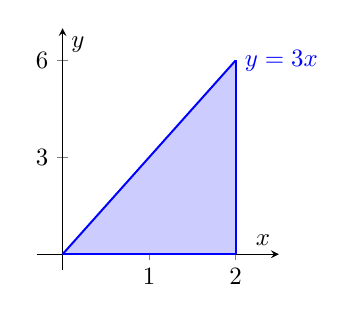
\begin{tikzpicture}[scale=0.9]
\begin{axis}[
  width=5cm, height=5cm,
  axis lines=middle,
  xlabel={$x$}, ylabel={$y$},
  xmin=-0.3, xmax=2.5, ymin=-0.5, ymax=7,
  xtick={1,2}, ytick={3,6},
  samples=50,
  clip=false
]
\addplot[fill=blue!20, draw=none, domain=0:2] {3*x} \closedcycle;
\addplot[thick, blue, domain=0:2] {3*x} node[right]{$y=3x$};
\addplot[thick, blue, domain=0:2] {0};
\draw[thick, blue] (axis cs:2,0) -- (axis cs:2,6);
\end{axis}
\end{tikzpicture}
\end{center}
The region $R$ is bounded below by $y=0$ and above by $y=3x$, with $0\le x\le 2$. As a Type I region, for each fixed $x\in[0,2]$, $y$ ranges from $0$ to $3x$.

The integral is:
\[
\boxed{\iint_R(x+y)\,dA = \int_0^2\int_0^{3x}(x+y)\,dy\,dx}.
\]

%%% PROBLEM 23 %%%
\item \textbf{Solution.}
\begin{center}
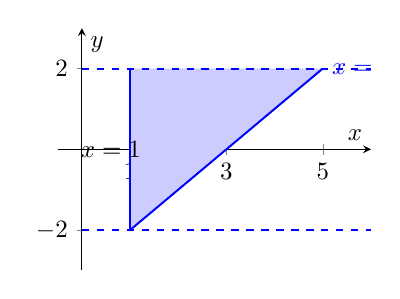
\begin{tikzpicture}[scale=0.9]
\begin{axis}[
  width=6cm, height=5cm,
  axis lines=middle,
  xlabel={$x$}, ylabel={$y$},
  xmin=-0.5, xmax=6, ymin=-3, ymax=3,
  xtick={1,3,5}, ytick={-2,0,2},
  samples=50
]
\addplot[fill=blue!20, draw=none] coordinates {(1,-2) (1,2) (5,2) (1,-2)} -- cycle;
\addplot[thick, blue] coordinates {(1,-2) (1,2)};
\addplot[thick, blue, domain=-2:2] ({x+3},{x}) node[right]{$x=y+3$};
\draw[thick, blue, dashed] (axis cs:0,-2) -- (axis cs:6,-2);
\draw[thick, blue, dashed] (axis cs:0,2) -- (axis cs:6,2);
\node at (axis cs:0.6,0) {$x=1$};
\end{axis}
\end{tikzpicture}
\end{center}
As a Type II region, $y$ ranges over $[-2,2]$, and for each fixed $y$, $x$ goes from the left boundary $x=1$ to the right boundary $x=y+3$.

The integral is:
\[
\boxed{\iint_R 5\,dA = \int_{-2}^{2}\int_1^{y+3}5\,dx\,dy}.
\]

%%% PROBLEM 24 %%%
\item \textbf{Solution.}
\begin{center}
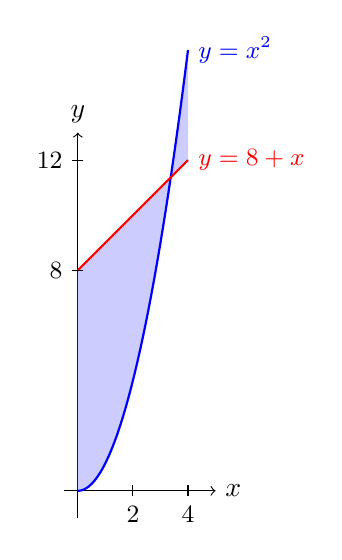
\begin{tikzpicture}[scale=0.35]
\draw[->] (-0.5,0) -- (5,0) node[right]{$x$};
\draw[->] (0,-1) -- (0,13) node[above]{$y$};
% Shaded region
\fill[blue!20] plot[domain=0:4,samples=40] (\x,{\x*\x}) -- (4,12) -- plot[domain=4:0,samples=40] (\x,{8+\x}) -- cycle;
% Curves
\draw[thick,blue] plot[domain=0:4,samples=40] (\x,{\x*\x}) node[right]{\small $y=x^2$};
\draw[thick,red] plot[domain=0:4,samples=2] (\x,{8+\x}) node[right]{\small $y=8+x$};
% Ticks
\foreach \x in {2,4} {\draw (\x,0.2) -- (\x,-0.2) node[below]{\small $\x$};}
\foreach \y in {8,12} {\draw (0.2,\y) -- (-0.2,\y) node[left]{\small $\y$};}
\end{tikzpicture}
\end{center}
\begin{enumerate}
\item $R$ is Type I because for each fixed $x\in[0,4]$, the variable $y$ ranges between two functions of $x$: from $y=x^2$ (below) to $y=8+x$ (above). The curves intersect when $x^2 = 8+x$, i.e., $x^2-x-8=0$, giving $x = \frac{1+\sqrt{33}}{2}\approx 3.37$. Since this is less than 4, we need to check that $x^2 \le 8+x$ for $x\in[0,4]$. At $x=4$: $x^2=16$ and $8+x=12$, so $x^2 > 8+x$. Thus the description $x^2 \le y \le 8+x$ is only valid for $0\le x\le \frac{1+\sqrt{33}}{2}$.

Correcting: $R$ as stated (with $x^2 \le y \le 8+x$ for $0\le x\le 4$) is Type I because the bounds on $y$ are given explicitly as functions of $x$.

\item As Type II: $y$ ranges from $\min(x^2)=0$ to $\max(8+x)=12$, so $y\in[0,12]$. For a given $y$, the left boundary comes from $x^2=y$ (i.e., $x=\sqrt{y}$) or $x=0$, and the right boundary comes from $y=8+x$ (i.e., $x=y-8$) or $x=4$. The region must be split:

As Type II, we solve for $x$: from $y=x^2$ we get $x=\sqrt{y}$, from $y=8+x$ we get $x=y-8$, and we have $0\le x\le 4$.

For $0\le y\le 8$: $x$ runs from $0$ to $\sqrt{y}$ (since $y-8<0$).

For $8 < y \le 9$: $x$ runs from $y-8$ to $\sqrt{y}$ (since both bounds are in $[0,4]$).

For $9 < y \le 12$: $x$ runs from $y-8$ to $4$ (since $\sqrt{y}>4$ would require $y>16$; actually $\sqrt{12}\approx 3.46<4$, so $x$ runs from $y-8$ to $\sqrt{y}$).

Let $x_0 = \frac{1+\sqrt{33}}{2}$. At the intersection, $y_0 = x_0^2$. For $y > y_0$, the parabola $x=\sqrt{y}$ exceeds the line $x=y-8$ but we also need $x\le 4$. At $y=12$: $\sqrt{12}<4$ and $y-8=4$, so $x$ from $\sqrt{y}$ to $4$---but this reverses. The Type II description requires careful case analysis, confirming that the Type I description is simpler.
\end{enumerate}

%%% PROBLEM 25 %%%
\item \textbf{Solution.}
The curves $y=x^2$ and $y=6-x$ intersect when $x^2 = 6-x$, i.e., $x^2+x-6=0$, giving $(x+3)(x-2)=0$, so $x=-3$ or $x=2$. On $[-1,3]$, the intersection within the interval is at $x=2$.

For $-1\le x\le 2$: $x^2 \le 6-x$, so the top curve is $y=6-x$ and the bottom is $y=x^2$.

For $2\le x\le 3$: $x^2 \ge 6-x$, so the top curve is $y=x^2$ and the bottom is $y=6-x$.

\[
A = \int_{-1}^2\bigl[(6-x)-x^2\bigr]\,dx + \int_2^3\bigl[x^2-(6-x)\bigr]\,dx.
\]

First integral:
\[
\int_{-1}^2(6-x-x^2)\,dx = \left[6x - \frac{x^2}{2}-\frac{x^3}{3}\right]_{-1}^2 = \frac{22}{3}+\frac{37}{6} = \frac{44+37}{6}=\frac{81}{6}=\frac{27}{2}.
\]

Second integral:
\begin{align*}
\int_2^3(x^2-6+x)\,dx &= \left[\frac{x^3}{3}-6x+\frac{x^2}{2}\right]_2^3 \\
&= \left(9-18+\frac{9}{2}\right)-\left(\frac{8}{3}-12+2\right) = \frac{9}{2}-9+12-\frac{8}{3}-2.
\end{align*}
Evaluating: at $x=3$, $9-18+9/2 = -9/2$; at $x=2$, $8/3-12+2 = -22/3$. Difference: $-9/2+22/3 = (-27+44)/6 = 17/6$.

Total area $= 27/2 + 17/6 = 81/6+17/6 = \boxed{\dfrac{98}{6} = \dfrac{49}{3}}$.

%%% PROBLEM 26 %%%
\item \textbf{Solution.}
\begin{enumerate}
\item \textbf{Type I ($dy\,dx$):} For $0\le x\le 2$, $y$ goes from $x$ to $4$:
\[
\int_0^2\int_x^4(1+xy)\,dy\,dx = \int_0^2\left[y+\frac{xy^2}{2}\right]_x^4 dx = \int_0^2\left[(4+8x)-\left(x+\frac{x^3}{2}\right)\right]dx
\]
\[
= \int_0^2\left(4+7x-\frac{x^3}{2}\right)dx = \left[4x+\frac{7x^2}{2}-\frac{x^4}{8}\right]_0^2 = 8+14-2 = \boxed{20}.
\]

\item \textbf{Type II ($dx\,dy$):} The region is $\{0\le x\le 2,\; x\le y\le 4\}$. For Type II, for fixed $y$: if $0\le y\le 2$, then $x$ ranges from $0$ to $y$; if $2\le y\le 4$, then $x$ ranges from $0$ to $2$.

\[
\int_0^2\int_0^y(1+xy)\,dx\,dy + \int_2^4\int_0^2(1+xy)\,dx\,dy.
\]

First part:
\[
\int_0^2\left[x+\frac{x^2 y}{2}\right]_0^y dy = \int_0^2\left(y+\frac{y^3}{2}\right)dy = \left[\frac{y^2}{2}+\frac{y^4}{8}\right]_0^2 = 2+2=4.
\]

Second part:
\[
\int_2^4\left[x+\frac{x^2 y}{2}\right]_0^2 dy = \int_2^4(2+2y)\,dy = \left[2y+y^2\right]_2^4 = (8+16)-(4+4)=16.
\]

Total: $4+16 = 20$.
\end{enumerate}

%%% PROBLEM 27 %%%
\item \textbf{Solution.}
\begin{center}
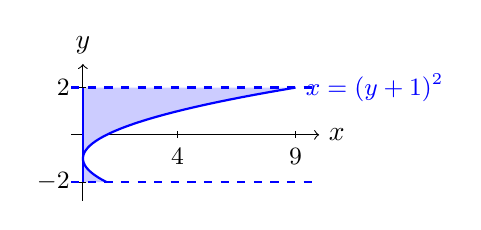
\begin{tikzpicture}[scale=0.3]
\draw[->] (-0.5,0) -- (10,0) node[right]{$x$};
\draw[->] (0,-2.8) -- (0,3) node[above]{$y$};
% Shaded region
\fill[blue!20] plot[domain=-2:2,samples=40] ({(\x+1)^2},\x) -- (0,2) -- (0,-2) -- cycle;
% Curve x=(y+1)^2
\draw[thick,blue] plot[domain=-2:2,samples=40] ({(\x+1)^2},\x) node[right]{\small $x=(y+1)^2$};
% Boundary lines
\draw[thick,blue] (0,-2) -- (0,2);
\draw[thick,blue,dashed] (-0.5,-2) -- (10,-2);
\draw[thick,blue,dashed] (-0.5,2) -- (10,2);
% Ticks
\draw (0.15,-2) -- (-0.15,-2) node[left]{\small $-2$};
\draw (0.15,2) -- (-0.15,2) node[left]{\small $2$};
\foreach \x in {4,9} {\draw (\x,0.15) -- (\x,-0.15) node[below]{\small $\x$};}
\end{tikzpicture}
\end{center}
The region is bounded by $x=0$, $y=-2$, $y=2$, $x=(y+1)^2$. For Type II: $y\in[-2,2]$, and for each $y$, $x$ ranges from $h_1(y)=0$ to $h_2(y)=(y+1)^2$.

\begin{align*}
&\int_{-2}^{2}\int_0^{(y+1)^2}(4-x-y)\,dx\,dy = \int_{-2}^2\left[4x-\frac{x^2}{2}-xy\right]_0^{(y+1)^2}dy \\
&= \int_{-2}^2\left[4(y+1)^2 - \frac{(y+1)^4}{2} - y(y+1)^2\right]dy.
\end{align*}

Let $u = y+1$, $y = u-1$, $dy = du$, and when $y=-2$, $u=-1$; when $y=2$, $u=3$:
\[
= \int_{-1}^3\left[4u^2 - \frac{u^4}{2}-(u-1)u^2\right]du = \int_{-1}^3\left[4u^2-\frac{u^4}{2}-u^3+u^2\right]du
\]
\[
= \int_{-1}^3\left(5u^2-u^3-\frac{u^4}{2}\right)du.
\]

\[
= \left[\frac{5u^3}{3}-\frac{u^4}{4}-\frac{u^5}{10}\right]_{-1}^3.
\]

At $u=3$: $\frac{5(27)}{3}-\frac{81}{4}-\frac{243}{10} = 45-\frac{81}{4}-\frac{243}{10}$.

Common denominator 20: $\frac{900-405-486}{20} = \frac{9}{20}$.

At $u=-1$: $\frac{5(-1)}{3}-\frac{1}{4}-\frac{-1}{10} = -\frac{5}{3}-\frac{1}{4}+\frac{1}{10}$.

Common denominator 60: $\frac{-100-15+6}{60} = \frac{-109}{60}$.

Result: $\frac{9}{20}+\frac{109}{60} = \frac{27+109}{60} = \frac{136}{60} = \boxed{\dfrac{34}{15}}$.

%%% PROBLEM 28 %%%
\item \textbf{Solution.}
\begin{center}
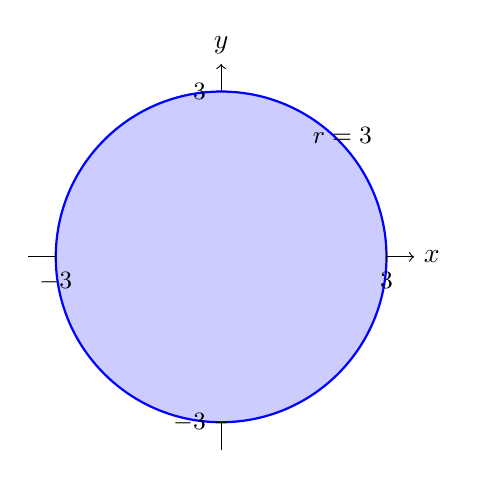
\begin{tikzpicture}[scale=0.7]
\draw[->] (-3.5,0) -- (3.5,0) node[right]{$x$};
\draw[->] (0,-3.5) -- (0,3.5) node[above]{$y$};
\fill[blue!20] (0,0) circle (3);
\draw[thick,blue] (0,0) circle (3);
\node at (2.2,2.2) {\small $r=3$};
\draw (3,0.1) -- (3,-0.1) node[below]{\small $3$};
\draw (-3,0.1) -- (-3,-0.1) node[below]{\small $-3$};
\draw (0.1,3) -- (-0.1,3) node[left]{\small $3$};
\draw (0.1,-3) -- (-0.1,-3) node[left]{\small $-3$};
\end{tikzpicture}
\end{center}
In polar coordinates, $x^2+y^2 = r^2$ and $dA = r\,dr\,d\theta$. The disk of radius 3: $0\le r\le 3$, $0\le\theta\le 2\pi$.

\[
\int_0^{2\pi}\int_0^3 r^2\cdot r\,dr\,d\theta = \int_0^{2\pi}\int_0^3 r^3\,dr\,d\theta = \int_0^{2\pi}\left[\frac{r^4}{4}\right]_0^3 d\theta = \int_0^{2\pi}\frac{81}{4}\,d\theta = \frac{81}{4}\cdot 2\pi = \boxed{\frac{81\pi}{2}}.
\]

%%% PROBLEM 29 %%%
\item \textbf{Solution.}
\begin{center}
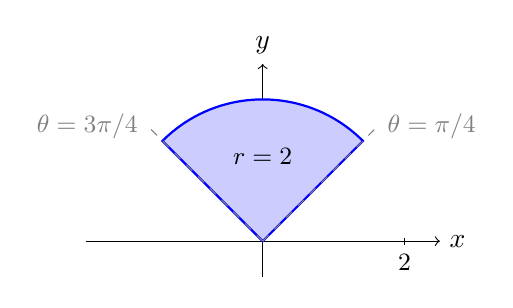
\begin{tikzpicture}[scale=0.9]
\draw[->] (-2.5,0) -- (2.5,0) node[right]{$x$};
\draw[->] (0,-0.5) -- (0,2.5) node[above]{$y$};
% Shaded sector
\fill[blue!20] (0,0) -- (45:2) arc (45:135:2) -- cycle;
\draw[thick,blue] (0,0) -- (45:2) arc (45:135:2) -- cycle;
% Labels
\draw[dashed,gray] (0,0) -- (45:2.3) node[right]{\small $\theta=\pi/4$};
\draw[dashed,gray] (0,0) -- (135:2.3) node[left]{\small $\theta=3\pi/4$};
\node at (90:1.2) {\small $r=2$};
\draw (2,0.05) -- (2,-0.05) node[below]{\small $2$};
\end{tikzpicture}
\end{center}
In polar coordinates: $x^2+y^2 = r^2$, $dA = r\,dr\,d\theta$.

The sector has $0\le r\le 2$, $\pi/4\le\theta\le 3\pi/4$. The integral becomes:
\[
\boxed{\iint_R(x^2+y^2)\,dA = \int_{\pi/4}^{3\pi/4}\int_0^2 r^2\cdot r\,dr\,d\theta = \int_{\pi/4}^{3\pi/4}\int_0^2 r^3\,dr\,d\theta}.
\]

%%% PROBLEM 30 %%%
\item \textbf{Solution.}
The annular region: $2\le r\le 3$, $0\le\theta\le 2\pi$. With $x = r\cos\theta$, $y = r\sin\theta$:

\[
\int_0^{2\pi}\!\int_2^3 (3+r\cos\theta+r\sin\theta)\,r\,dr\,d\theta.
\]

Expand:
\[
= \int_0^{2\pi}\!\int_2^3\bigl(3r + r^2\cos\theta + r^2\sin\theta\bigr)\,dr\,d\theta.
\]

The terms $r^2\cos\theta$ and $r^2\sin\theta$ integrate to 0 over $[0,2\pi]$ in $\theta$ since $\int_0^{2\pi}\cos\theta\,d\theta = \int_0^{2\pi}\sin\theta\,d\theta = 0$.

Remaining:
\[
\int_0^{2\pi}\int_2^3 3r\,dr\,d\theta = 2\pi\cdot 3\left[\frac{r^2}{2}\right]_2^3 = 2\pi\cdot 3\cdot\frac{9-4}{2} = 2\pi\cdot\frac{15}{2} = \boxed{15\pi}.
\]

%%% PROBLEM 31 %%%
\item \textbf{Solution.}
\begin{enumerate}
\item The closed region $R$ is bounded by the parabola $y=x^2$ from $x=0$ to $x=1$ and the quarter-circle $x^2+y^2=1$ in the first quadrant (from $(1,0)$ back to $(0,1)$ is above the parabola for $0<x<1$).

The parabola $y=x^2$ and the quarter-circle $x^2+y^2=1$ intersect at $(0,0)$ (approximately) and $(x_0,y_0)$ where $x^2+x^4=1$. In the first quadrant, the region between them is awkward in a single coordinate system. Splitting:
\begin{itemize}
\item $R_1$: between $y=x^2$ and $y=\sqrt{1-x^2}$ --- best in Cartesian since the parabola has a simple Cartesian form.
\item $R_2$: the quarter-disk portion that doesn't overlap $R_1$ --- best in polar since it is part of a circle.
\end{itemize}

\item Let $x_0$ solve $x^2+x^4=1$, so $x_0^2 = \frac{-1+\sqrt{5}}{2}$.

$R_1$ (Cartesian): $0\le x\le x_0$, $x^2\le y\le\sqrt{1-x^2}$:
\[
\iint_{R_1}(1+x^2+y^2)\,dA = \int_0^{x_0}\int_{x^2}^{\sqrt{1-x^2}}(1+x^2+y^2)\,dy\,dx.
\]

$R_2$ (Polar): the quarter-disk from $\theta=0$ to $\theta=\pi/2$, $r$ from $0$ to $1$, minus $R_1$. Alternatively, $R$ is the region in the first quadrant between $y=x^2$ and the circle, and the full integral is simply:
\[
\iint_R(1+x^2+y^2)\,dA = \int_0^{x_0}\int_{x^2}^{\sqrt{1-x^2}}(1+x^2+y^2)\,dy\,dx.
\]
If we want a polar piece for the quarter-disk portion beyond $x_0$, note that for $x_0\le x$, the parabola rises above the circle, so the region is entirely captured by the single Cartesian integral above.
\end{enumerate}

%%% PROBLEM 32 %%%
\item \textbf{Solution.}
\begin{center}
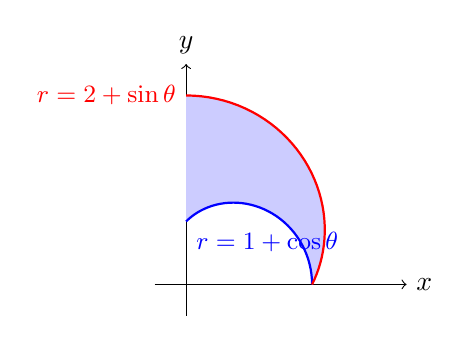
\begin{tikzpicture}[scale=0.8]
\draw[->] (-0.5,0) -- (3.5,0) node[right]{$x$};
\draw[->] (0,-0.5) -- (0,3.5) node[above]{$y$};
% Shaded region between r=1+cos(theta) and r=2+sin(theta) for 0<=theta<=pi/2
\fill[blue!20]
  plot[domain=0:90,samples=40] ({(1+cos(\x))*cos(\x)},{(1+cos(\x))*sin(\x)})
  -- plot[domain=90:0,samples=40] ({(2+sin(\x))*cos(\x)},{(2+sin(\x))*sin(\x)})
  -- cycle;
% Inner curve r=1+cos(theta)
\draw[thick,blue] plot[domain=0:90,samples=40] ({(1+cos(\x))*cos(\x)},{(1+cos(\x))*sin(\x)})
  node[below right]{\small $r=1+\cos\theta$};
% Outer curve r=2+sin(theta)
\draw[thick,red] plot[domain=0:90,samples=40] ({(2+sin(\x))*cos(\x)},{(2+sin(\x))*sin(\x)})
  node[left]{\small $r=2+\sin\theta$};
\end{tikzpicture}
\end{center}
In polar coordinates, $\sqrt{x^2+y^2} = r$ and $dA = r\,dr\,d\theta$, so the integrand becomes $r\cdot r\,dr\,d\theta = r^2\,dr\,d\theta$.

For $0\le\theta\le\pi/2$, the inner radius is $r = 1+\cos\theta$ and the outer radius is $r = 2+\sin\theta$.

\[
\boxed{\iint_R\sqrt{x^2+y^2}\,dA = \int_0^{\pi/2}\int_{1+\cos\theta}^{2+\sin\theta} r^2\,dr\,d\theta}.
\]

%%% PROBLEM 33 %%%
\item \textbf{Solution.}
\begin{center}
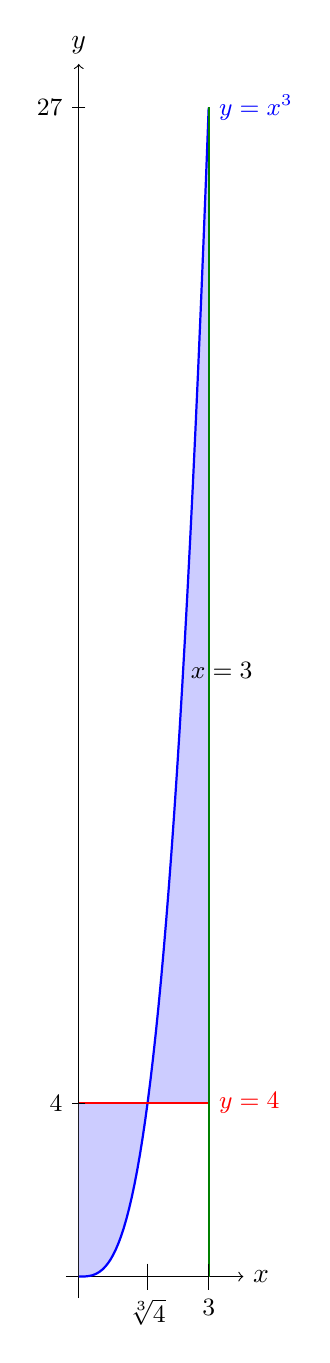
\begin{tikzpicture}[scale=0.55]
\draw[->] (-0.3,0) -- (3.8,0) node[right]{$x$};
\draw[->] (0,-0.5) -- (0,28) node[above]{$y$};
% Shaded region: two parts
% Part 1: 0<=x<=4^{1/3}, x^3<=y<=4
\fill[blue!20] plot[domain=0:1.587,samples=30] (\x,{\x*\x*\x}) -- (1.587,4) -- (0,4) -- (0,0) -- cycle;
% Part 2: 4^{1/3}<=x<=3, 4<=y<=x^3
\fill[blue!20] (1.587,4) -- plot[domain=1.587:3,samples=30] (\x,{\x*\x*\x}) -- (3,4) -- cycle;
% Curves
\draw[thick,blue] plot[domain=0:3,samples=50] (\x,{\x*\x*\x}) node[right]{\small $y=x^3$};
\draw[thick,red] (0,4) -- (3,4) node[right]{\small $y=4$};
\draw[thick,green!50!black] (3,0) -- (3,27);
% Ticks
\draw (3,0.3) -- (3,-0.3) node[below]{\small $3$};
\draw (1.587,0.3) -- (1.587,-0.3) node[below]{\small $\sqrt[3]{4}$};
\draw (0.15,4) -- (-0.15,4) node[left]{\small $4$};
\draw (0.15,27) -- (-0.15,27) node[left]{\small $27$};
\node at (3.3,14) {\small $x=3$};
\end{tikzpicture}
\end{center}
The region in the first quadrant is bounded by $y=x^3$, $y=4$, and $x=3$.

The curve $y=x^3$ reaches $y=4$ at $x=4^{1/3}\approx 1.587$. The region bounded by $y=x^3$, $y=4$, and $x=3$ in the first quadrant splits into two subregions:

For $0\le x\le 4^{1/3}$: the region is between $y=x^3$ and $y=4$.

For $4^{1/3}\le x\le 3$: $x^3\ge 4$, so the curve $y=x^3$ is above $y=4$. The region is between $y=4$ and $y=x^3$ (with $x^3$ on top) bounded by $x=3$.

So two Type I subregions:

$R_1$: $0\le x\le 4^{1/3}$, $x^3\le y\le 4$:
\[
\int_0^{4^{1/3}}\int_{x^3}^4(2x+y)\,dy\,dx.
\]

$R_2$: $4^{1/3}\le x\le 3$, $4\le y\le x^3$:
\[
\int_{4^{1/3}}^3\int_4^{x^3}(2x+y)\,dy\,dx.
\]

The full integral is the sum of these two integrals.

%%% PROBLEM 34 %%%
\item \textbf{Solution.}
The plate occupies $0\le x\le 3$, $0\le y\le x^2$, with $\rho(x,y) = 5+x$.

\begin{enumerate}
\item Total mass:
\[
M = \int_0^3\int_0^{x^2}(5+x)\,dy\,dx = \int_0^3(5+x)\cdot x^2\,dx = \int_0^3(5x^2+x^3)\,dx.
\]
\[
= \left[\frac{5x^3}{3}+\frac{x^4}{4}\right]_0^3 = 45+\frac{81}{4} = \frac{180+81}{4} = \frac{261}{4}.
\]

\item Moments:
\[
M_x = \int_0^3\int_0^{x^2}y(5+x)\,dy\,dx = \int_0^3(5+x)\frac{x^4}{2}\,dx = \frac{1}{2}\int_0^3(5x^4+x^5)\,dx
\]
\[
= \frac{1}{2}\left[x^5+\frac{x^6}{6}\right]_0^3 = \frac{1}{2}\left(243+\frac{729}{6}\right) = \frac{1}{2}\cdot\frac{1458+729}{6} = \frac{2187}{12} = \frac{729}{4}.
\]

\[
M_y = \int_0^3\int_0^{x^2}x(5+x)\,dy\,dx = \int_0^3 x(5+x)\cdot x^2\,dx = \int_0^3(5x^3+x^4)\,dx
\]
\[
= \left[\frac{5x^4}{4}+\frac{x^5}{5}\right]_0^3 = \frac{5\cdot81}{4}+\frac{243}{5} = \frac{405}{4}+\frac{243}{5} = \frac{2025+972}{20} = \frac{2997}{20}.
\]

\item Center of mass:
\begin{align*}
\bar{x} &= \frac{M_y}{M} = \frac{2997/20}{261/4} = \frac{2997}{20}\cdot\frac{4}{261} = \frac{2997}{1305}\\
&= \frac{999}{435} = \frac{333}{145}\approx 2.297.
\end{align*}
\[
\bar{y} = \frac{M_x}{M} = \frac{729/4}{261/4} = \frac{729}{261} = \frac{243}{87} = \frac{81}{29}\approx 2.793.
\]
\end{enumerate}

%%% PROBLEM 35 %%%
\item \textbf{Solution.}
\begin{enumerate}
\item The cardioid $r = 2+2\cos\theta$ traces out for $\theta\in[0,2\pi]$. The area is:
\[
A = \int_0^{2\pi}\int_0^{2+2\cos\theta}r\,dr\,d\theta = \int_0^{2\pi}\frac{(2+2\cos\theta)^2}{2}\,d\theta = \int_0^{2\pi}\frac{4(1+\cos\theta)^2}{2}\,d\theta
\]
\[
= 2\int_0^{2\pi}(1+2\cos\theta+\cos^2\theta)\,d\theta = 2\left[2\pi+0+\pi\right] = 6\pi.
\]

\item In Cartesian, the cardioid $r=2+2\cos\theta$ becomes $\sqrt{x^2+y^2} = 2 + \frac{2x}{\sqrt{x^2+y^2}}$, i.e., $x^2+y^2 = 2\sqrt{x^2+y^2}+2x$. Squaring and rearranging gives a complicated implicit equation. Describing the bounds as explicit functions $y = f(x)$ requires solving this quartic---far messier than the clean polar integral. This demonstrates why polar coordinates are more convenient for regions defined by polar equations like cardioids.
\end{enumerate}

%%% PROBLEM 36 %%%
\item \textbf{Solution.}
\begin{enumerate}
\item The region $R$ is in the first quadrant ($x\ge 0$, $y\ge 0$), inside the circle $x^2+y^2=4$ (radius 2), and below the line $y=2-x$. Note that $y=2-x$ intersects the circle when $x^2+(2-x)^2=4$, i.e., $2x^2-4x=0$, giving $x=0$ or $x=2$. So the line connects $(0,2)$ to $(2,0)$, exactly the chord of the circle. The region bounded by $x=0$, $y=0$, the circle, and the line is actually the region in the first quadrant between the line $y=2-x$ and the circular arc.

The line $y=2-x$ lies inside the circle (since at the midpoint $(1,1)$, $1+1=2<4$). So the region between the line (below) and the arc (above) is one piece, plus the triangular region below the line.

The region is bounded by all four curves simultaneously. The simplest interpretation: $R$ is the region in the first quadrant that is inside the circle and above the line $y=2-x$---the region between the chord and the arc.

Alternatively, $R$ could be the region below both the circle and the line. Let us take $R$ as the region with $x\ge 0$, $y\ge 0$, $x^2+y^2\le 4$, and $y\le 2-x$ (the triangular region under the chord). In that case, $R$ is a triangle with vertices $(0,0)$, $(2,0)$, $(0,2)$.

For the more interesting case where $R$ is between the chord and the arc: $x\ge 0$, $y\ge 0$, $x^2+y^2\le 4$, $y\ge 2-x$:

\item \textbf{Split approach:} Use polar coordinates for the circular part. In polar, the circle is $r=2$ and the line $x+y=2$ becomes $r(\cos\theta+\sin\theta)=2$, i.e., $r = \frac{2}{\cos\theta+\sin\theta}$.

The full integral over $R$ (between chord and arc):
\[
\iint_R(x+y)\,dA = \int_0^{\pi/2}\int_{2/(\cos\theta+\sin\theta)}^{2}(r\cos\theta+r\sin\theta)\,r\,dr\,d\theta
\]
\[
= \int_0^{\pi/2}\int_{2/(\cos\theta+\sin\theta)}^{2}r^2(\cos\theta+\sin\theta)\,dr\,d\theta.
\]
This is a clean single integral in polar coordinates.
\end{enumerate}

%%% PROBLEM 37 %%%
\item \textbf{Solution.}
\begin{enumerate}
\item The total mass is:
\[
M = \iint_R \rho_0\,dA = \int_0^3\int_0^2 5\,dy\,dx.
\]

\item Evaluating:
\[
M = 5\int_0^3\int_0^2 dy\,dx = 5\cdot 3\cdot 2 = \boxed{30\text{ kg}}.
\]
\end{enumerate}

%%% PROBLEM 38 %%%
\item \textbf{Solution.}
The triangle has vertices $(0,0)$, $(4,0)$, $(4,3)$. The hypotenuse goes from $(0,0)$ to $(4,3)$: $y = \frac{3x}{4}$.

\begin{enumerate}
\item As a Type I region: $0\le x\le 4$, $0\le y\le 3x/4$.
\[
M = \int_0^4\int_0^{3x/4}2\,dy\,dx = 2\cdot\frac{3}{4}\int_0^4 x\,dx = \frac{3}{2}\cdot 8 = \boxed{12\text{ kg}}.
\]

(Check: area of triangle $= \frac{1}{2}\cdot 4\cdot 3 = 6$, times $\rho_0=2$ gives $12$.)

\item Center of mass:
\begin{align*}
\bar{x} &= \frac{1}{M}\int_0^4\int_0^{3x/4}2x\,dy\,dx = \frac{1}{12}\cdot 2\int_0^4 x\cdot\frac{3x}{4}\,dx\\
&= \frac{1}{12}\cdot\frac{3}{2}\int_0^4 x^2\,dx = \frac{1}{12}\cdot\frac{3}{2}\cdot\frac{64}{3} = \frac{1}{12}\cdot 32 = \frac{8}{3}.
\end{align*}

\begin{align*}
\bar{y} &= \frac{1}{M}\int_0^4\int_0^{3x/4}2y\,dy\,dx = \frac{1}{12}\cdot 2\int_0^4\frac{1}{2}\left(\frac{3x}{4}\right)^2 dx\\
&= \frac{1}{12}\int_0^4\frac{9x^2}{16}\,dx = \frac{1}{12}\cdot\frac{9}{16}\cdot\frac{64}{3} = \frac{1}{12}\cdot 12 = 1.
\end{align*}

So $(\bar{x},\bar{y}) = \boxed{\left(\frac{8}{3}, 1\right)}$.

\item Since $\bar{x} = 8/3 \approx 2.67 > 2$ (more than halfway along the $x$-base of length 4), this is because the triangle widens as $x$ increases: the height at position $x$ is $3x/4$, which grows linearly with $x$. Thus more area (and hence more mass, since density is uniform) is concentrated toward larger $x$-values, pulling the centroid past the midpoint.
\end{enumerate}

%%% PROBLEM 39 %%%
\item \textbf{Solution.}
\begin{enumerate}
\item $\displaystyle M = \int_0^2\int_0^3(5+x)\,dy\,dx$.

\item Evaluating:
\[
M = \int_0^2(5+x)\cdot 3\,dx = 3\int_0^2(5+x)\,dx = 3\left[5x+\frac{x^2}{2}\right]_0^2 = 3\left(10+2\right) = 3\cdot 12 = \boxed{36\text{ g}}.
\]
\end{enumerate}

%%% PROBLEM 40 %%%
\item \textbf{Solution.}
\begin{enumerate}
\item The region $R$ is in the first quadrant bounded by $x=0$, $y=0$, $y=4-x^2$. The parabola meets the $x$-axis at $x=2$.

Area of $R$:
\[
A = \int_0^2(4-x^2)\,dx = \left[4x-\frac{x^3}{3}\right]_0^2 = 8-\frac{8}{3} = \frac{16}{3}.
\]

Average temperature:
\[
T_{\text{avg}} = \frac{1}{A}\int_0^2\int_0^{4-x^2}(10+xy)\,dy\,dx.
\]

\item Inner integral:
\[
\int_0^{4-x^2}(10+xy)\,dy = \left[10y+\frac{xy^2}{2}\right]_0^{4-x^2} = 10(4-x^2)+\frac{x(4-x^2)^2}{2}.
\]

Expanding: $10(4-x^2) = 40-10x^2$ and $\frac{x(16-8x^2+x^4)}{2} = 8x-4x^3+\frac{x^5}{2}$.

Outer integral:
\begin{align*}
&\int_0^2\left(40-10x^2+8x-4x^3+\frac{x^5}{2}\right)dx \\
&= \left[40x-\frac{10x^3}{3}+4x^2-x^4+\frac{x^6}{12}\right]_0^2 \\
&= 80-\frac{80}{3}+16-16+\frac{64}{12} = 80-\frac{80}{3}+\frac{16}{3} = 80-\frac{64}{3} = \frac{240-64}{3} = \frac{176}{3}.
\end{align*}

\[
T_{\text{avg}} = \frac{3}{16}\cdot\frac{176}{3} = \frac{176}{16} = \boxed{11\,{}^\circ\text{C}}.
\]
\end{enumerate}

%%% PROBLEM 41 %%%
\item \textbf{Solution.}
In polar coordinates, $y = r\sin\theta$ and $dA = r\,dr\,d\theta$. The semicircular region: $0\le r\le 3$, $0\le\theta\le\pi$.

\[
I_x = \iint_R y^2\,dA = \int_0^\pi\int_0^3 (r\sin\theta)^2\cdot r\,dr\,d\theta = \int_0^\pi\int_0^3 r^3\sin^2\theta\,dr\,d\theta.
\]

\[
= \left(\int_0^3 r^3\,dr\right)\!\left(\int_0^\pi\sin^2\theta\,d\theta\right) = \frac{81}{4}\cdot\frac{\pi}{2} = \boxed{\frac{81\pi}{8}}.
\]

This is indeed simpler in polar than in Cartesian, where we would need $\int_{-3}^3\int_0^{\sqrt{9-x^2}}y^2\,dy\,dx$ with a more complex antiderivative.

%%% PROBLEM 42 %%%
\item \textbf{Solution.}
In polar: $x^2+y^2 = r^2$, disk of radius $R$: $0\le r\le R$, $0\le\theta\le 2\pi$.

\[
I_z = \rho_0\int_0^{2\pi}\int_0^R r^2\cdot r\,dr\,d\theta = \rho_0\int_0^{2\pi}\int_0^R r^3\,dr\,d\theta = \rho_0\cdot 2\pi\cdot\frac{R^4}{4} = \boxed{\rho_0\pi\frac{R^4}{2}}. \qed
\]

%%% PROBLEM 43 %%%
\item \textbf{Solution.}
\begin{enumerate}
\item $\displaystyle M = \int_0^{2\pi}\int_0^2(4+r)\,r\,dr\,d\theta$.

\item Evaluating the $r$-integral:
\[
\int_0^2(4r+r^2)\,dr = \left[2r^2+\frac{r^3}{3}\right]_0^2 = 8+\frac{8}{3} = \frac{32}{3}.
\]
\[
M = 2\pi\cdot\frac{32}{3} = \boxed{\frac{64\pi}{3}}.
\]

\item Average density:
\[
\rho_{\text{avg}} = \frac{M}{\text{Area}} = \frac{64\pi/3}{\pi\cdot 4} = \frac{64}{12} = \boxed{\frac{16}{3}}.
\]
\end{enumerate}

%%% PROBLEM 44 %%%
\item \textbf{Solution.}
\begin{enumerate}
\item With $z = x^2+3y^2$:
\[
\frac{\partial z}{\partial x} = 2x, \qquad \frac{\partial z}{\partial y} = 6y.
\]

\item The surface area integral is:
\[
A = \iint_R\sqrt{1+(2x)^2+(6y)^2}\,dA = \boxed{\int_0^2\int_0^1\sqrt{1+4x^2+36y^2}\,dy\,dx}.
\]

This integral does not simplify to a closed form easily and would typically be evaluated numerically.
\end{enumerate}

%%% PROBLEM 45 %%%
\item \textbf{Solution.}
For the cone $z = \sqrt{x^2+y^2}$:
\[
\frac{\partial z}{\partial x} = \frac{x}{\sqrt{x^2+y^2}}, \qquad \frac{\partial z}{\partial y} = \frac{y}{\sqrt{x^2+y^2}}.
\]
\[
1+\left(\frac{\partial z}{\partial x}\right)^2+\left(\frac{\partial z}{\partial y}\right)^2 = 1+\frac{x^2}{x^2+y^2}+\frac{y^2}{x^2+y^2} = 1+1 = 2.
\]

The cone lies below $z=3$ when $\sqrt{x^2+y^2}\le 3$, i.e., over the disk $x^2+y^2\le 9$.

\[
A = \iint_{x^2+y^2\le 9}\sqrt{2}\,dA = \sqrt{2}\cdot\pi(3)^2 = \boxed{9\pi\sqrt{2}}.
\]

%%% PROBLEM 46 %%%
\item \textbf{Solution.}
For $z = \sqrt{4-x^2-y^2}$:
\[
\frac{\partial z}{\partial x} = \frac{-x}{\sqrt{4-x^2-y^2}}, \qquad \frac{\partial z}{\partial y} = \frac{-y}{\sqrt{4-x^2-y^2}}.
\]
\[
1+\frac{x^2}{4-x^2-y^2}+\frac{y^2}{4-x^2-y^2} = \frac{4-x^2-y^2+x^2+y^2}{4-x^2-y^2} = \frac{4}{4-x^2-y^2}.
\]

In polar coordinates over $x^2+y^2\le 4$:
\[
A = \int_0^{2\pi}\int_0^2\frac{2}{\sqrt{4-r^2}}\,r\,dr\,d\theta = 2\pi\int_0^2\frac{2r}{\sqrt{4-r^2}}\,dr.
\]

Let $u = 4-r^2$, $du = -2r\,dr$:
\[
= 2\pi\int_4^0\frac{-2\,du}{2\sqrt{u}} = 2\pi\cdot 2\left[\sqrt{u}\right]_0^4 = 2\pi\cdot 2\cdot 2 = 8\pi.
\]

The geometric formula for a hemisphere of radius 2 gives $2\pi r^2 = 2\pi(4) = 8\pi$.

$\boxed{A = 8\pi}$.

%%% PROBLEM 47 %%%
\item \textbf{Solution.}
\begin{center}
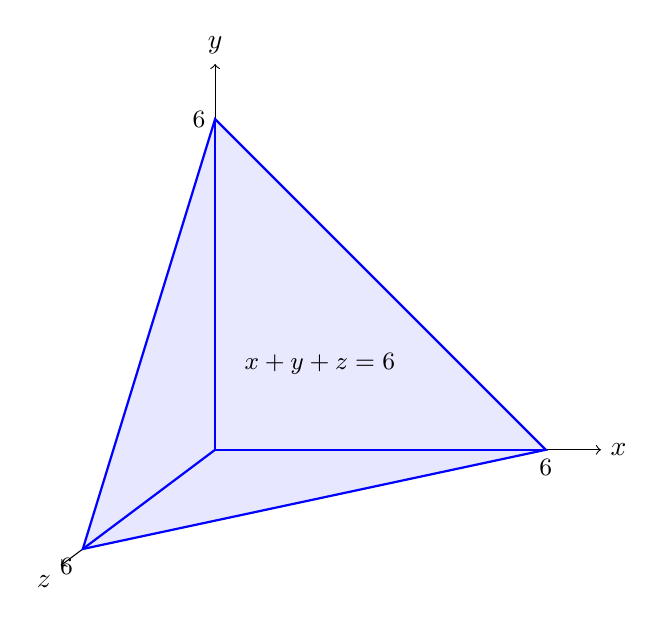
\begin{tikzpicture}[scale=0.7, z={(-.4,-.3)}]
% Axes
\draw[->] (0,0,0) -- (7,0,0) node[right]{$x$};
\draw[->] (0,0,0) -- (0,7,0) node[above]{$y$};
\draw[->] (0,0,0) -- (0,0,7) node[below left]{$z$};
% Tetrahedron faces (shaded)
\fill[blue!15,opacity=0.6] (6,0,0) -- (0,6,0) -- (0,0,6) -- cycle;
\fill[blue!10,opacity=0.4] (0,0,0) -- (6,0,0) -- (0,0,6) -- cycle;
\fill[blue!10,opacity=0.4] (0,0,0) -- (0,6,0) -- (0,0,6) -- cycle;
% Edges
\draw[thick,blue] (6,0,0) -- (0,6,0) -- (0,0,6) -- cycle;
\draw[thick,blue] (0,0,0) -- (6,0,0);
\draw[thick,blue] (0,0,0) -- (0,6,0);
\draw[thick,blue] (0,0,0) -- (0,0,6);
% Labels
\node[below] at (6,0,0) {\small $6$};
\node[left] at (0,6,0) {\small $6$};
\node[below left] at (0,0,6) {\small $6$};
\node at (2.5,2,1.5) {\small $x+y+z=6$};
\end{tikzpicture}
\end{center}
The first octant region bounded by $z=0$, $x=0$, $y=0$, and $x+y+z=6$ (so $z = 6-x-y$). With $x,y,z\ge 0$: $x+y\le 6$.

Choosing order $dz\,dy\,dx$: for fixed $x,y$, $z$ ranges from $0$ to $6-x-y$; for fixed $x$, $y$ ranges from $0$ to $6-x$; $x$ ranges from $0$ to $6$.

\[
\boxed{\iiint_E(2xy-z)\,dV = \int_0^6\int_0^{6-x}\int_0^{6-x-y}(2xy-z)\,dz\,dy\,dx}.
\]

%%% PROBLEM 48 %%%
\item \textbf{Solution.}
\begin{center}
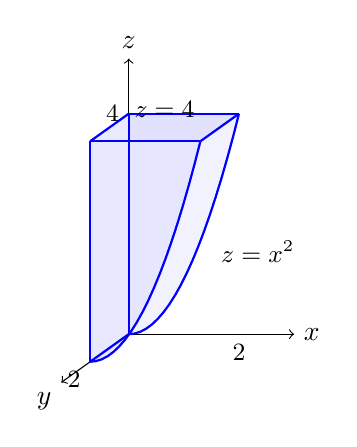
\begin{tikzpicture}[scale=0.7, z={(-.35,-.25)}]
% Axes
\draw[->] (0,0,0) -- (3,0,0) node[right]{$x$};
\draw[->] (0,0,0) -- (0,5,0) node[above]{$z$};
\draw[->] (0,0,0) -- (0,0,3.5) node[below left]{$y$};
% Back face (x-z plane at y=2): parabola z=x^2 up to z=4
\fill[blue!15,opacity=0.6] (0,0,2) -- plot[domain=0:2,samples=20] (\x,{\x*\x},2) -- (2,4,2) -- (0,4,2) -- cycle;
% Front face (x-z plane at y=0): parabola z=x^2 up to z=4
\fill[blue!10,opacity=0.5] (0,0,0) -- plot[domain=0:2,samples=20] (\x,{\x*\x},0) -- (2,4,0) -- (0,4,0) -- cycle;
% Top face z=4
\fill[blue!20,opacity=0.4] (0,4,0) -- (2,4,0) -- (2,4,2) -- (0,4,2) -- cycle;
% Edges
\draw[thick,blue] plot[domain=0:2,samples=20] (\x,{\x*\x},0);
\draw[thick,blue] plot[domain=0:2,samples=20] (\x,{\x*\x},2);
\draw[thick,blue] (0,0,0) -- (0,0,2);
\draw[thick,blue] (2,4,0) -- (2,4,2);
\draw[thick,blue] (0,4,0) -- (0,4,2);
\draw[thick,blue] (0,4,0) -- (2,4,0);
\draw[thick,blue] (0,4,2) -- (2,4,2);
\draw[thick,blue] (0,0,0) -- (0,4,0);
\draw[thick,blue] (0,0,2) -- (0,4,2);
% Labels
\node[below] at (2,0,0) {\small $2$};
\node[left] at (0,4,0) {\small $4$};
\node[below left] at (0,0,2) {\small $2$};
\node[right] at (1.5,1.5,0) {\small $z=x^2$};
\node[above] at (1,4,1) {\small $z=4$};
\end{tikzpicture}
\end{center}
The region $E$ is bounded by $z=x^2$ (below), $z=4$ (above), $x=0$, and $y=2$ (with $y\ge 0$ implied). Since $z=x^2\le 4$ requires $|x|\le 2$, and $x=0$ is one boundary, we need $0\le x\le 2$, $0\le y\le 2$, $x^2\le z\le 4$.

\begin{align*}
V &= \int_0^2\int_0^2\int_{x^2}^4 dz\,dy\,dx = \int_0^2\int_0^2(4-x^2)\,dy\,dx = \int_0^2 2(4-x^2)\,dx \\
&= 2\left[4x-\frac{x^3}{3}\right]_0^2 = 2\left(8-\frac{8}{3}\right) = \boxed{\frac{32}{3}}.
\end{align*}

%%% PROBLEM 49 %%%
\item \textbf{Solution.}
The tetrahedron: $x,y,z\ge 0$, $2x+3y+z\le 6$, so $z\le 6-2x-3y$.

For the base in the $xy$-plane: $2x+3y\le 6$, $x\ge 0$, $y\ge 0$, so $0\le x\le 3$, $0\le y\le (6-2x)/3$.

\[
I = \int_0^3\int_0^{(6-2x)/3}\int_0^{6-2x-3y}(x^2+yz)\,dz\,dy\,dx.
\]

Inner integral ($z$):
\[
\int_0^{6-2x-3y}(x^2+yz)\,dz = x^2(6-2x-3y)+\frac{y(6-2x-3y)^2}{2}.
\]

Let $a = 6-2x-3y$. The inner integral is $x^2 a + ya^2/2$.

Middle integral ($y$), with $a = 6-2x-3y$: Let $b = 6-2x$, so $a = b-3y$.

\[
\int_0^{b/3}\left[x^2(b-3y)+\frac{y(b-3y)^2}{2}\right]dy.
\]

First term: $x^2\int_0^{b/3}(b-3y)\,dy = x^2\left[by-\frac{3y^2}{2}\right]_0^{b/3} = x^2\left(\frac{b^2}{3}-\frac{b^2}{6}\right) = \frac{x^2 b^2}{6}$.

Second term: $\frac{1}{2}\int_0^{b/3}y(b-3y)^2\,dy$. Expand $(b-3y)^2 = b^2-6by+9y^2$:
\[
\frac{1}{2}\int_0^{b/3}(b^2 y-6by^2+9y^3)\,dy = \frac{1}{2}\left[\frac{b^2 y^2}{2}-2by^3+\frac{9y^4}{4}\right]_0^{b/3}.
\]
At $y=b/3$: $\frac{b^4}{18}-\frac{2b^4}{27}+\frac{b^4}{36}$. Common denominator 108: $\frac{6b^4-8b^4+3b^4}{108} = \frac{b^4}{108}$.

So the second term is $\frac{b^4}{216}$.

Middle integral $= \frac{x^2 b^2}{6}+\frac{b^4}{216}$ where $b = 6-2x$.

Outer integral ($x$):
\[
I = \int_0^3\left[\frac{x^2(6-2x)^2}{6}+\frac{(6-2x)^4}{216}\right]dx.
\]

Let $u = 6-2x$, $x = (6-u)/2$, $dx = -du/2$. When $x=0$, $u=6$; when $x=3$, $u=0$.

\[
I = \int_6^0\left[\frac{(6-u)^2 u^2}{4\cdot 6}+\frac{u^4}{216}\right]\left(-\frac{du}{2}\right) = \frac{1}{2}\int_0^6\left[\frac{(6-u)^2 u^2}{24}+\frac{u^4}{216}\right]du.
\]

\[
= \frac{1}{48}\int_0^6(6-u)^2 u^2\,du + \frac{1}{432}\int_0^6 u^4\,du.
\]

For $\int_0^6(6-u)^2 u^2\,du$: expand $(6-u)^2 u^2 = (36-12u+u^2)u^2 = 36u^2-12u^3+u^4$:
\begin{align*}
&= \left[12u^3-3u^4+\frac{u^5}{5}\right]_0^6 = 12(216)-3(1296)+\frac{7776}{5} \\
&= 2592-3888+1555.2 = 259.2 = \frac{1296}{5}.
\end{align*}

For $\int_0^6 u^4\,du = \frac{6^5}{5} = \frac{7776}{5}$.

\[
I = \frac{1}{48}\cdot\frac{1296}{5}+\frac{1}{432}\cdot\frac{7776}{5} = \frac{1296}{240}+\frac{7776}{2160} = \frac{27}{5}+\frac{18}{5} = \frac{45}{5} = \boxed{9}.
\]

(Here $\frac{1296}{240} = \frac{27}{5}$ and $\frac{7776}{2160} = \frac{18}{5}$, confirming $\frac{27}{5}+\frac{18}{5} = 9$.)

%%% PROBLEM 50 %%%
\item \textbf{Solution.}
The integral with the given bounds is:
\[
\boxed{\int_{-1}^{2}\int_0^{\pi}\int_0^3 (3r^2+z)\,r\,dr\,d\theta\,dz}.
\]
Equivalently (reordering):
\[
\int_0^{\pi}\int_0^3\int_{-1}^{2}(3r^2+z)\,r\,dz\,dr\,d\theta.
\]

The bounds are: $r\in[0,3]$, $\theta\in[0,\pi]$, $z\in[-1,2]$.

%%% PROBLEM 51 %%%
\item \textbf{Solution.}
In spherical coordinates: $x^2+y^2+z^2 = \rho^2$, $dV = \rho^2\sin\phi\,d\rho\,d\phi\,d\theta$.

Ball of radius 4: $0\le\rho\le 4$, $0\le\phi\le\pi$, $0\le\theta\le 2\pi$.

\[
\iiint_E\rho^2\,dV = \int_0^{2\pi}\int_0^{\pi}\int_0^4\rho^2\cdot\rho^2\sin\phi\,d\rho\,d\phi\,d\theta = \int_0^{2\pi}d\theta\int_0^{\pi}\sin\phi\,d\phi\int_0^4\rho^4\,d\rho.
\]

\[
= 2\pi\cdot\bigl[-\cos\phi\bigr]_0^\pi\cdot\left[\frac{\rho^5}{5}\right]_0^4 = 2\pi\cdot 2\cdot\frac{1024}{5} = \boxed{\frac{4096\pi}{5}}.
\]

%%% PROBLEM 52 %%%
\item \textbf{Solution.}
The two spheres are $\rho = 2$ and $x^2+y^2+(z-2)^2=4$. Expanding the second: $x^2+y^2+z^2-4z+4=4$, so $\rho^2-4\rho\cos\phi=0$ (since $z=\rho\cos\phi$), giving $\rho = 4\cos\phi$.

The intersection region is where both $\rho\le 2$ and $\rho\le 4\cos\phi$. These spheres intersect when $2 = 4\cos\phi$, i.e., $\cos\phi = 1/2$, so $\phi = \pi/3$.

The intersection region (interior to both spheres) is:
\begin{itemize}
\item For $0\le\phi\le\pi/3$: the sphere $\rho=2$ is the binding constraint (since $4\cos\phi\ge 2$), so $0\le\rho\le 2$.
\item For $\pi/3\le\phi\le\pi/2$: the sphere $\rho=4\cos\phi$ is binding (since $4\cos\phi\le 2$), so $0\le\rho\le 4\cos\phi$.
\end{itemize}
And $0\le\theta\le 2\pi$. (For $\phi>\pi/2$, $4\cos\phi<0$, so there is no contribution.)

The volume integral is:
\[
\boxed{V = \int_0^{2\pi}\int_0^{\pi/3}\int_0^{2}\rho^2\sin\phi\,d\rho\,d\phi\,d\theta + \int_0^{2\pi}\int_{\pi/3}^{\pi/2}\int_0^{4\cos\phi}\rho^2\sin\phi\,d\rho\,d\phi\,d\theta}.
\]

%%% PROBLEM 53 %%%
\item \textbf{Solution.}
We use spherical coordinates. The first octant of the sphere $x^2+y^2+z^2\le 9$: $0\le\rho\le 3$, $0\le\phi\le\pi/2$, $0\le\theta\le\pi/2$.

With $\rho(x,y,z) = 3x = 3\rho\sin\phi\cos\theta$:

\begin{align*}
I &= \int_0^{\pi/2}\int_0^{\pi/2}\int_0^3 3\rho\sin\phi\cos\theta\cdot\rho^2\sin\phi\,d\rho\,d\phi\,d\theta \\
&= 3\int_0^{\pi/2}\cos\theta\,d\theta\int_0^{\pi/2}\sin^2\phi\,d\phi\int_0^3\rho^3\,d\rho.
\end{align*}

\[
= 3\cdot[\sin\theta]_0^{\pi/2}\cdot\frac{\pi}{4}\cdot\frac{81}{4} = 3\cdot 1\cdot\frac{\pi}{4}\cdot\frac{81}{4} = \boxed{\frac{243\pi}{16}}.
\]

%%% PROBLEM 54 %%%
\item \textbf{Solution.}
Transform to polar: $x = r\cos\theta$, $y = r\sin\theta$, Jacobian $= r$. The disk $x^2+y^2\le 4$ becomes $0\le r\le 2$, $0\le\theta\le 2\pi$. Also $4-x^2-y^2 = 4-r^2$.

\[
\boxed{\iint_R(4-x^2-y^2)\,dA = \int_0^{2\pi}\int_0^2(4-r^2)\,r\,dr\,d\theta}.
\]

%%% PROBLEM 55 %%%
\item \textbf{Solution.}
The parallelogram has vertices $(0,0)$, $(2,0)$, $(3,2)$, $(1,2)$. The edges from $(0,0)$ are to $(2,0)$ (direction $(2,0)$) and to $(1,2)$ (direction $(1,2)$).

Let $u = x - y/2$ and $v = y$. Then the vertices map to:
\begin{itemize}
\item $(0,0)\to(0,0)$
\item $(2,0)\to(2,0)$
\item $(3,2)\to(2,2)$
\item $(1,2)\to(0,2)$
\end{itemize}

So the rectangle is $0\le u\le 2$, $0\le v\le 2$. The inverse transformation: $x = u+v/2$, $y = v$.

Jacobian: $\frac{\partial(x,y)}{\partial(u,v)} = \begin{vmatrix} 1 & 1/2 \\ 0 & 1\end{vmatrix} = 1$.

Observe the edges of $R$. Along the bottom ($y=0$): $x$ goes from $0$ to $2$. Along the top ($y=2$): $x$ goes from $1$ to $3$. Along the left: from $(0,0)$ to $(1,2)$, so $x = y/2$. Along the right: from $(2,0)$ to $(3,2)$, so $x = y/2+2$.

Let $u = x - y/2$, $v = y$. Then $R$ maps to $0\le u\le 2$, $0\le v\le 2$, the Jacobian is $|J| = 1$, and $x + y = u + 3v/2$.

The transformed integral is:
\[
\boxed{\int_0^2\int_0^2 \exp\!\left(\left(u + \frac{3v}{2}\right)^2\right)\,du\,dv, \quad |J| = 1}.
\]

(Note: while this doesn't fully separate the integrand, the region is now a rectangle, which is the primary simplification sought.)

%%% PROBLEM 56 %%%
\item \textbf{Solution.}
\begin{enumerate}
\item The Jacobian:
\[
J = \frac{\partial(x,y)}{\partial(u,v)} = \begin{vmatrix} \partial x/\partial u & \partial x/\partial v \\ \partial y/\partial u & \partial y/\partial v\end{vmatrix} = \begin{vmatrix} 2 & 3 \\ 1 & -2\end{vmatrix} = -4-3 = -7.
\]
So $|J| = \boxed{7}$.

\item In terms of $u,v$: $x+2y = (2u+3v)+2(u-2v) = 4u-v$.
\[
\boxed{\iint_R(x+2y)\,dx\,dy = \int_0^3\int_0^2(4u-v)\cdot 7\,dv\,du = 7\int_0^3\int_0^2(4u-v)\,dv\,du}.
\]
\end{enumerate}

%%% PROBLEM 57 %%%
\item \textbf{Solution.}
With $x = r^2\cos\theta$, $y = r^2\sin\theta$:

\[
J = \frac{\partial(x,y)}{\partial(r,\theta)} = \begin{vmatrix} 2r\cos\theta & -r^2\sin\theta \\ 2r\sin\theta & r^2\cos\theta\end{vmatrix} = 2r^3\cos^2\theta+2r^3\sin^2\theta = 2r^3.
\]

Also $\sqrt{x^2+y^2} = \sqrt{r^4\cos^2\theta+r^4\sin^2\theta} = r^2$.

Over the region $0\le r\le 1$, $0\le\theta\le 2\pi$:
\[
\boxed{\iint_R\sqrt{x^2+y^2}\,dx\,dy = \int_0^{2\pi}\int_0^1 r^2\cdot 2r^3\,dr\,d\theta = \int_0^{2\pi}\int_0^1 2r^5\,dr\,d\theta}.
\]

Evaluating: $\int_0^1 2r^5\,dr = \frac{1}{3}$, so the integral $= 2\pi/3$.

%%% PROBLEM 58 %%%
\item \textbf{Solution.}
The transformation $u = (x-y)/\sqrt{2}$, $v = (x+y)/\sqrt{2}$ gives $x = (u+v)/\sqrt{2}$, $y = (v-u)/\sqrt{2}$.

Jacobian: $\frac{\partial(x,y)}{\partial(u,v)} = \begin{vmatrix} 1/\sqrt{2} & 1/\sqrt{2} \\ -1/\sqrt{2} & 1/\sqrt{2}\end{vmatrix} = \frac{1}{2}+\frac{1}{2} = 1$.

The square $R$ has vertices $(0,0)$, $(2,0)$, $(2,2)$, $(0,2)$. Under the transformation:
\begin{itemize}
\item $(0,0)\to(0,0)$
\item $(2,0)\to(\sqrt{2},\sqrt{2})$
\item $(2,2)\to(0,2\sqrt{2})$
\item $(0,2)\to(-\sqrt{2},\sqrt{2})$
\end{itemize}

The image is a square in the $uv$-plane rotated $45°$, with vertices as listed---a diamond with diagonals along the axes from $-\sqrt{2}$ to $\sqrt{2}$ in $u$ and $0$ to $2\sqrt{2}$ in $v$.

The new region $R'$ in $(u,v)$: For $0\le v\le\sqrt{2}$, $u\in[-v,v]$; for $\sqrt{2}\le v\le 2\sqrt{2}$, $u\in[-(2\sqrt{2}-v),2\sqrt{2}-v]$.

Since the integrand is 1 and $|J|=1$:
\[
\boxed{\iint_R 1\,dx\,dy = \int_0^{\sqrt{2}}\int_{-v}^{v}1\,du\,dv + \int_{\sqrt{2}}^{2\sqrt{2}}\int_{-(2\sqrt{2}-v)}^{2\sqrt{2}-v}1\,du\,dv}.
\]

(The result is $4$, matching the area of the original square.)

%%% PROBLEM 59 %%%
\item \textbf{Solution.}
In cylindrical coordinates: $x = r\cos\theta$, $y = r\sin\theta$, $z = z$, and $dV = r\,dr\,d\theta\,dz$.

The cylinder $x^2+y^2\le 4$: $0\le r\le 2$, $0\le\theta\le 2\pi$, $0\le z\le 5$.

The integrand: $x+2y-z = r\cos\theta+2r\sin\theta-z$.

\[
\boxed{\iiint_E(x+2y-z)\,dV = \int_0^{2\pi}\int_0^2\int_0^5(r\cos\theta+2r\sin\theta-z)\,r\,dz\,dr\,d\theta}.
\]

%%% PROBLEM 60 %%%
\item \textbf{Solution.}
The parallelogram has vertices $(0,0)$, $(2,0)$, $(1+a,2+a)$, $(3+a,2+a)$.

Edge vectors from $(0,0)$: to $(2,0)$, direction $\mathbf{e}_1 = (2,0)$; to $(1+a,2+a)$, direction $\mathbf{e}_2 = (1+a,2+a)$.

Note: $(2,0)+(1+a,2+a) = (3+a,2+a)$, confirming the fourth vertex.

Let $u,v\in[0,1]$ parameterize: $(x,y) = u(2,0)+v(1+a,2+a)$, so $x = 2u+(1+a)v$, $y = (2+a)v$.

From $y = (2+a)v$: $v = y/(2+a)$. Then $u = (x-(1+a)v)/2$.

Jacobian: $|J| = \begin{vmatrix}2 & 1+a \\ 0 & 2+a\end{vmatrix} = 2(2+a)$.

So $dx\,dy = 2(2+a)\,du\,dv$.

Also $x+y = 2u+(1+a)v+(2+a)v = 2u+(3+2a)v$.

\[
\boxed{\iint_R(x+y)\,dx\,dy = 2(2+a)\int_0^1\int_0^1\bigl[2u+(3+2a)v\bigr]\,du\,dv}.
\]

%%% PROBLEM 61 %%%
\item \textbf{Solution.}
In spherical coordinates: $x = \rho\sin\phi\cos\theta$, $y = \rho\sin\phi\sin\theta$, $z = \rho\cos\phi$.

Then $x^2+y^2+z^2 = \rho^2$ and $dV = \rho^2\sin\phi\,d\rho\,d\phi\,d\theta$.

The sphere $x^2+y^2+z^2\le 9$: $0\le\rho\le 3$, $0\le\phi\le\pi$, $0\le\theta\le 2\pi$.

\[
\iiint_E\rho^2\,dV = \int_0^{2\pi}\int_0^\pi\int_0^3\rho^2\cdot\rho^2\sin\phi\,d\rho\,d\phi\,d\theta.
\]

Step by step:
\[
\int_0^3\rho^4\,d\rho = \frac{243}{5}, \qquad \int_0^\pi\sin\phi\,d\phi = 2, \qquad \int_0^{2\pi}d\theta = 2\pi.
\]

\[
= 2\pi\cdot 2\cdot\frac{243}{5} = \boxed{\frac{972\pi}{5}}.
\]

%%% PROBLEM 62 %%%
\item \textbf{Solution.}
The change of variables is defined by $u = x-y$, $v = y-2z$, $w = x+z$.

Solving for $(x,y,z)$ in terms of $(u,v,w)$: From $u = x-y$ and $w = x+z$, we get $z = w-x$. From $v = y-2z = y-2(w-x) = y-2w+2x$, and $y = x-u$, so $v = x-u-2w+2x = 3x-u-2w$, giving $x = \frac{u+v+2w}{3}$.

Then $y = x-u = \frac{u+v+2w}{3}-u = \frac{v+2w-2u}{3}$ and $z = w-x = w-\frac{u+v+2w}{3} = \frac{-u-v+w}{3}$.

The Jacobian matrix $\frac{\partial(x,y,z)}{\partial(u,v,w)}$:
\[
\begin{pmatrix} 1/3 & 1/3 & 2/3 \\ -2/3 & 1/3 & 2/3 \\ -1/3 & -1/3 & 1/3\end{pmatrix}.
\]

Determinant (expanding along the first row):
\[
\frac{1}{3}\left(\frac{1}{9}+\frac{2}{9}\right)-\frac{1}{3}\left(-\frac{2}{9}+\frac{2}{9}\right)+\frac{2}{3}\left(\frac{2}{9}+\frac{1}{9}\right) = \frac{1}{3}\cdot\frac{3}{9}+0+\frac{2}{3}\cdot\frac{3}{9} = \frac{1}{9}+\frac{2}{9} = \frac{1}{3}.
\]

So $|J| = 1/3$. Also:
\[
4xyz = 4\cdot\frac{u+v+2w}{3}\cdot\frac{v+2w-2u}{3}\cdot\frac{w-u-v}{3}.
\]

The integral in $(u,v,w)$-space is:
\[
\boxed{\int_0^2\int_0^1\int_0^3 4\cdot\frac{(u+v+2w)(v+2w-2u)(w-u-v)}{27}\cdot\frac{1}{3}\,dw\,dv\,du}.
\]
\[
= \frac{4}{81}\int_0^2\int_0^1\int_0^3(u+v+2w)(v+2w-2u)(w-u-v)\,dw\,dv\,du.
\]

%%% PROBLEM 63 %%%
\item \textbf{Solution.}
\begin{enumerate}
\item The Jacobian matrix:
\[
J = \frac{\partial(x,y,z)}{\partial(\mu,\nu,z)} = \begin{pmatrix} a\sinh\mu\cos\nu & -a\cosh\mu\sin\nu & 0 \\ a\cosh\mu\sin\nu & a\sinh\mu\cos\nu & 0 \\ 0 & 0 & 1\end{pmatrix}.
\]

\item The determinant:
\begin{align*}
|J| &= 1\cdot\bigl(a\sinh\mu\cos\nu\cdot a\sinh\mu\cos\nu - (-a\cosh\mu\sin\nu)(a\cosh\mu\sin\nu)\bigr)\\
&= a^2\sinh^2\mu\cos^2\nu + a^2\cosh^2\mu\sin^2\nu \\
&= a^2\bigl(\sinh^2\mu\cos^2\nu + \cosh^2\mu\sin^2\nu\bigr).
\end{align*}

Using $\cosh^2\mu = 1+\sinh^2\mu$:
\[
= a^2\bigl(\sinh^2\mu\cos^2\nu + \sin^2\nu + \sinh^2\mu\sin^2\nu\bigr) = a^2(\sinh^2\mu + \sin^2\nu).
\]

The volume element becomes:
\[
\boxed{dV = a^2(\sinh^2\mu + \sin^2\nu)\,d\mu\,d\nu\,dz}.
\]

The factor $a^2(\sinh^2\mu+\sin^2\nu)$ acts as a scale factor that accounts for the non-uniform stretching of the elliptic cylindrical coordinate system. Near $\mu=0$ and $\nu=0$ (or $\pi$), the factor is small, reflecting the compression near the foci of the ellipses.
\end{enumerate}

%%% PROBLEM 64 %%%
\item \textbf{Solution.}
Set up the cone with apex at the origin and base at $z=3$. At height $z$, the radius is $r = z/3$ (since at $z=3$, $r=1$).

Using cylindrical coordinates:
\[
M = \int_0^{2\pi}\int_0^3\int_0^{z/3} kz\cdot r\,dr\,dz\,d\theta.
\]

Inner integral ($r$):
\[
\int_0^{z/3}kz\cdot r\,dr = kz\cdot\frac{r^2}{2}\Big|_0^{z/3} = kz\cdot\frac{z^2}{18} = \frac{kz^3}{18}.
\]

Middle integral ($z$):
\[
\int_0^3\frac{kz^3}{18}\,dz = \frac{k}{18}\cdot\frac{81}{4} = \frac{81k}{72} = \frac{9k}{8}.
\]

Outer integral ($\theta$):
\[
M = 2\pi\cdot\frac{9k}{8} = \boxed{\frac{9\pi k}{4}}.
\]

%%% PROBLEM 65 %%%
\item \textbf{Solution.}
In spherical coordinates: $x = \rho\sin\phi\cos\theta$, $y = \rho\sin\phi\sin\theta$, $z = \rho\cos\phi$, $dV = \rho^2\sin\phi\,d\rho\,d\phi\,d\theta$.

Hemisphere of radius 2, $z\ge 0$: $0\le\rho\le 2$, $0\le\phi\le\pi/2$, $0\le\theta\le 2\pi$.

Density: $\rho(x,y,z) = 1+z^2 = 1+\rho^2\cos^2\phi$.

\[
\boxed{M = \int_0^{2\pi}\int_0^{\pi/2}\int_0^2(1+\rho^2\cos^2\phi)\,\rho^2\sin\phi\,d\rho\,d\phi\,d\theta}.
\]

%%% PROBLEM 66 %%%
\item \textbf{Solution.}
\begin{enumerate}
\item Total mass:
\[
M = \int_0^1\int_0^2\int_0^3(x+y+z)\,dz\,dy\,dx.
\]

Evaluating:
\[
\int_0^3(x+y+z)\,dz = 3(x+y)+\frac{9}{2} = 3x+3y+\frac{9}{2}.
\]
\[
\int_0^2\left(3x+3y+\frac{9}{2}\right)dy = 6x+6+9 = 6x+15.
\]
\[
M = \int_0^1(6x+15)\,dx = 3+15 = \boxed{18}.
\]

\item The moment $M_{xy}$ (for the $z$-coordinate):
\[
M_{xy} = \int_0^1\int_0^2\int_0^3 z(x+y+z)\,dz\,dy\,dx.
\]
\[
\int_0^3 z(x+y+z)\,dz = (x+y)\frac{9}{2}+9 = \frac{9(x+y)}{2}+9.
\]
\[
\int_0^2\left(\frac{9(x+y)}{2}+9\right)dy = 9x+9+18 = 9x+27.
\]
\[
M_{xy} = \int_0^1(9x+27)\,dx = \frac{9}{2}+27 = \frac{63}{2}.
\]

\[
\bar{z} = \frac{M_{xy}}{M} = \frac{63/2}{18} = \frac{63}{36} = \boxed{\frac{7}{4}}.
\]
\end{enumerate}

%%% PROBLEM 67 %%%
\item \textbf{Solution.}
Let $u = x/3$, $v = y/2$, $w = z$. Then the ellipsoid $x^2/9+y^2/4+z^2\le 1$ becomes $u^2+v^2+w^2\le 1$ (a unit sphere).

The Jacobian: $x=3u$, $y=2v$, $z=w$, so $\frac{\partial(x,y,z)}{\partial(u,v,w)} = 3\cdot 2\cdot 1 = 6$.

The density: $\rho = \sqrt{x^2+y^2+z^2} = \sqrt{9u^2+4v^2+w^2}$.

The total mass:
\[
\boxed{M = 6\int\!\!\!\int\!\!\!\int_{u^2+v^2+w^2\le 1}\sqrt{9u^2+4v^2+w^2}\,du\,dv\,dw}.
\]

(This can be further converted to spherical coordinates in $(u,v,w)$-space, though the integrand $\sqrt{9\sin^2\alpha\cos^2\beta+4\sin^2\alpha\sin^2\beta+\cos^2\alpha}$ would depend on angles and not simplify to a closed form easily.)

%%% PROBLEM 68 %%%
\item \textbf{Solution.}
\begin{enumerate}
\item The total force $\mathbf{F}_{\text{total}} = \iiint_E \mathbf{F}\,dV = \left(\iiint_E yz\,dV,\;\iiint_E xz\,dV,\;\iiint_E xy\,dV\right)$.

Using cylindrical coordinates ($x=r\cos\theta$, $y=r\sin\theta$), the cylinder is $0\le r\le 2$, $0\le\theta\le 2\pi$, $0\le z\le 5$.

\textbf{$x$-component:} $\iiint yz\,dV = \int_0^{2\pi}\int_0^2\int_0^5 (r\sin\theta)(z)\,r\,dz\,dr\,d\theta$. The $\theta$-integral contains $\int_0^{2\pi}\sin\theta\,d\theta = 0$. So the $x$-component is $\mathbf{0}$.

\textbf{$y$-component:} Similarly contains $\int_0^{2\pi}\cos\theta\,d\theta = 0$. So the $y$-component is $\mathbf{0}$.

\textbf{$z$-component:} $\iiint xy\,dV = \int_0^{2\pi}\int_0^2\int_0^5 r^2\cos\theta\sin\theta\cdot r\,dz\,dr\,d\theta$. The $\theta$-integral: $\int_0^{2\pi}\cos\theta\sin\theta\,d\theta = \frac{1}{2}\int_0^{2\pi}\sin 2\theta\,d\theta = 0$. So the $z$-component is $\mathbf{0}$.

Therefore $\boxed{\mathbf{F}_{\text{total}} = \mathbf{0}}$.

(This is expected by symmetry: the cylinder is symmetric under $\theta\to\theta+\pi$, and each component of $\mathbf{F}$ is an odd function under this rotation.)

\item The work done per unit time (power) is:
\[
W = \iiint_E \mathbf{F}\cdot\mathbf{v}\,dV = \iiint_E (yz\cdot x + xz\cdot y + xy\cdot z)\,dV = \iiint_E 3xyz\,dV.
\]

In cylindrical: $3xyz = 3r\cos\theta\cdot r\sin\theta\cdot z = 3r^2 z\cos\theta\sin\theta$.
\[
W = \int_0^{2\pi}\int_0^2\int_0^5 3r^2 z\cos\theta\sin\theta\cdot r\,dz\,dr\,d\theta.
\]

Again, $\int_0^{2\pi}\cos\theta\sin\theta\,d\theta = 0$, so $\boxed{W = 0}$.
\end{enumerate}

%%% PROBLEM 69 %%%
\item \textbf{Solution.}
The moment of inertia about the $z$-axis is $I_z = \iiint_E (x^2+y^2)\rho_0\,dV$.

In spherical coordinates: $x^2+y^2 = \rho^2\sin^2\phi$, $dV = \rho^2\sin\phi\,d\rho\,d\phi\,d\theta$.

\[
I_z = \rho_0\int_0^{2\pi}\int_0^\pi\int_0^R\rho^2\sin^2\phi\cdot\rho^2\sin\phi\,d\rho\,d\phi\,d\theta = \rho_0\int_0^{2\pi}d\theta\int_0^\pi\sin^3\phi\,d\phi\int_0^R\rho^4\,d\rho.
\]

\[
\int_0^{2\pi}d\theta = 2\pi, \quad \int_0^R\rho^4\,d\rho = \frac{R^5}{5}.
\]

\begin{align*}
\int_0^\pi\sin^3\phi\,d\phi &= \int_0^\pi(1-\cos^2\phi)\sin\phi\,d\phi
= \left[-\cos\phi+\frac{\cos^3\phi}{3}\right]_0^\pi \\
&= \left(1-\frac{1}{3}\right)-\left(-1+\frac{1}{3}\right) = \frac{4}{3}.
\end{align*}

\[
I_z = \rho_0\cdot 2\pi\cdot\frac{4}{3}\cdot\frac{R^5}{5} = \boxed{\frac{8\pi\rho_0 R^5}{15}}.
\]

Since the total mass is $M = \rho_0\cdot\frac{4}{3}\pi R^3$, this equals $\frac{2}{5}MR^2$, the well-known result.

%%% PROBLEM 70 %%%
\item \textbf{Solution.}
\begin{enumerate}
\item The tetrahedron: $x,y,z\ge 0$, $x+2y+3z\le 6$.

Bounds: $0\le x\le 6$, $0\le y\le (6-x)/2$, $0\le z\le (6-x-2y)/3$.

\[
M = \int_0^6\int_0^{(6-x)/2}\int_0^{(6-x-2y)/3}(2x+5y+z)\,dz\,dy\,dx.
\]

Let $a = 6-x-2y$. Inner integral:
\[
\int_0^{a/3}(2x+5y+z)\,dz = (2x+5y)\frac{a}{3}+\frac{a^2}{18}.
\]

Middle integral ($y$), with $a = 6-x-2y$, let $b = 6-x$:
\[
\int_0^{b/2}\left[(2x+5y)\frac{b-2y}{3}+\frac{(b-2y)^2}{18}\right]dy.
\]

First part: $\frac{1}{3}\int_0^{b/2}(2x+5y)(b-2y)\,dy$.

Expand: $(2x+5y)(b-2y) = 2xb-4xy+5by-10y^2$.
\[
\frac{1}{3}\left[2xby-2xy^2+\frac{5by^2}{2}-\frac{10y^3}{3}\right]_0^{b/2}.
\]
At $y = b/2$: $2xb\cdot\frac{b}{2}-2x\cdot\frac{b^2}{4}+\frac{5b}{2}\cdot\frac{b^2}{4}-\frac{10}{3}\cdot\frac{b^3}{8} = xb^2-\frac{xb^2}{2}+\frac{5b^3}{8}-\frac{5b^3}{12}$.
$= \frac{xb^2}{2}+\frac{15b^3-10b^3}{24} = \frac{xb^2}{2}+\frac{5b^3}{24}$.

So first part $= \frac{1}{3}\left(\frac{xb^2}{2}+\frac{5b^3}{24}\right) = \frac{xb^2}{6}+\frac{5b^3}{72}$.

Second part: $\frac{1}{18}\int_0^{b/2}(b-2y)^2\,dy$. Let $t = b-2y$:
$= \frac{1}{18}\cdot\frac{1}{2}\int_0^b t^2\,dt = \frac{1}{36}\cdot\frac{b^3}{3} = \frac{b^3}{108}$.

Middle integral $= \frac{xb^2}{6}+\frac{5b^3}{72}+\frac{b^3}{108} = \frac{xb^2}{6}+b^3\left(\frac{5}{72}+\frac{1}{108}\right) = \frac{xb^2}{6}+b^3\cdot\frac{15+2}{216} = \frac{xb^2}{6}+\frac{17b^3}{216}$.

Outer integral ($x$), $b = 6-x$:
\[
M = \int_0^6\left[\frac{x(6-x)^2}{6}+\frac{17(6-x)^3}{216}\right]dx.
\]

Let $u = 6-x$, $x = 6-u$, $dx = -du$:
\[
M = \int_0^6\left[\frac{(6-u)u^2}{6}+\frac{17u^3}{216}\right]du.
\]

$= \int_0^6\left[u^2-\frac{u^3}{6}+\frac{17u^3}{216}\right]du = \int_0^6\left[u^2+u^3\left(\frac{17}{216}-\frac{1}{6}\right)\right]du = \int_0^6\left[u^2+u^3\cdot\frac{17-36}{216}\right]du$.

$= \int_0^6\left[u^2-\frac{19u^3}{216}\right]du = \left[\frac{u^3}{3}-\frac{19u^4}{864}\right]_0^6 = \frac{216}{3}-\frac{19\cdot 1296}{864} = 72-\frac{24624}{864}$.

$\frac{24624}{864}$: simplify by dividing by 24: $\frac{1026}{36} = \frac{171}{6} = \frac{57}{2} = 28.5$.

$M = 72-28.5 = \boxed{43.5 = \frac{87}{2}}$.

\item For the center of mass, we need $M_x = \iiint x\rho\,dV$, $M_y = \iiint y\rho\,dV$, $M_z = \iiint z\rho\,dV$ where $\rho = 2x+5y+z$.

We compute each moment integral in turn.

For $\bar{x}$:
\[
\iiint_E x(2x+5y+z)\,dV = \iiint_E(2x^2+5xy+xz)\,dV.
\]

Using $u = 6-x$ substitution after integrating over $z$ and $y$:

Inner ($z$): $\int_0^{a/3}x(2x+5y+z)\,dz = x(2x+5y)\frac{a}{3}+\frac{xa^2}{18}$, where $a=6-x-2y$.

Middle ($y$): $\int_0^{b/2}\left[\frac{x(2x+5y)(b-2y)}{3}+\frac{x(b-2y)^2}{18}\right]dy$ where $b=6-x$.

$= x\left[\frac{1}{3}\int_0^{b/2}(2x+5y)(b-2y)\,dy+\frac{1}{18}\int_0^{b/2}(b-2y)^2\,dy\right]$.

From before: $= x\left[\frac{xb^2}{6}+\frac{5b^3}{72}+\frac{b^3}{108}\right] = x\left[\frac{xb^2}{6}+\frac{17b^3}{216}\right] = \frac{x^2 b^2}{6}+\frac{17xb^3}{216}$.

Outer: $\int_0^6\left[\frac{x^2(6-x)^2}{6}+\frac{17x(6-x)^3}{216}\right]dx$.

With $u=6-x$, $x=6-u$:
$= \int_0^6\left[\frac{(6-u)^2 u^2}{6}+\frac{17(6-u)u^3}{216}\right]du$.

First term: $\frac{1}{6}\int_0^6(36u^2-12u^3+u^4)\,du = \frac{1}{6}\left[12u^3-3u^4+\frac{u^5}{5}\right]_0^6$
$= \frac{1}{6}\left(2592-3888+\frac{7776}{5}\right) = \frac{1}{6}\cdot\frac{12960-19440+7776}{5} = \frac{1}{6}\cdot\frac{1296}{5} = \frac{216}{5} = 43.2$.

Second term: $\frac{17}{216}\int_0^6(6u^3-u^4)\,du = \frac{17}{216}\left[\frac{6u^4}{4}-\frac{u^5}{5}\right]_0^6 = \frac{17}{216}\left(\frac{6\cdot 1296}{4}-\frac{7776}{5}\right)$
$= \frac{17}{216}\left(1944-1555.2\right) = \frac{17}{216}\cdot\frac{9720-7776}{5} = \frac{17}{216}\cdot\frac{1944}{5} = \frac{17\cdot 9}{5} = \frac{153}{5}$.

So $\iiint x\rho\,dV = \frac{216+153}{5} = \frac{369}{5}$.

$\bar{x} = \frac{369/5}{87/2} = \frac{369}{5}\cdot\frac{2}{87} = \frac{738}{435} = \frac{246}{145} = \frac{246}{145}$.

Simplify: $\gcd(246,145)$. $246 = 1\cdot 145+101$, $145=1\cdot 101+44$, $101=2\cdot 44+13$, $44=3\cdot 13+5$, $13=2\cdot 5+3$, $5=1\cdot 3+2$, $3=1\cdot 2+1$. So $\gcd=1$. Thus $\bar{x} = \frac{246}{145}$.

For $\bar{y}$: We need $\iiint y(2x+5y+z)\,dV$.

Inner ($z$): $\int_0^{a/3}y(2x+5y+z)\,dz = y(2x+5y)\frac{a}{3}+\frac{ya^2}{18}$, $a=b-2y$, $b=6-x$.

Middle ($y$):
\[
\int_0^{b/2}\left[\frac{y(2x+5y)(b-2y)}{3}+\frac{y(b-2y)^2}{18}\right]dy.
\]

First part: expanding $y(2x+5y)(b-2y) = (2xy+5y^2)(b-2y) = 2xby-4xy^2+5by^2-10y^3$:

$\frac{1}{3}\left[xby^2-\frac{4xy^3}{3}+\frac{5by^3}{3}-\frac{10y^4}{4}\right]_0^{b/2}$.

At $y=b/2$: $\frac{xb^3}{4}-\frac{xb^3}{6}+\frac{5b^4}{24}-\frac{10b^4}{64} = xb^3\left(\frac{1}{4}-\frac{1}{6}\right)+b^4\left(\frac{5}{24}-\frac{5}{32}\right) = \frac{xb^3}{12}+b^4\cdot\frac{20-15}{96} = \frac{xb^3}{12}+\frac{5b^4}{96}$.

Multiply by $1/3$: $\frac{xb^3}{36}+\frac{5b^4}{288}$.

Second part: $\frac{1}{18}\int_0^{b/2}y(b-2y)^2\,dy = \frac{1}{18}\int_0^{b/2}(b^2 y-4by^2+4y^3)\,dy$

$= \frac{1}{18}\left[\frac{b^2 y^2}{2}-\frac{4by^3}{3}+y^4\right]_0^{b/2} = \frac{1}{18}\left(\frac{b^4}{8}-\frac{b^4}{6}+\frac{b^4}{16}\right)$.

$= \frac{b^4}{18}\left(\frac{1}{8}-\frac{1}{6}+\frac{1}{16}\right) = \frac{b^4}{18}\cdot\frac{6-8+3}{48} = \frac{b^4}{18}\cdot\frac{1}{48} = \frac{b^4}{864}$.

Middle integral $= \frac{xb^3}{36}+\frac{5b^4}{288}+\frac{b^4}{864} = \frac{xb^3}{36}+b^4\left(\frac{15+1}{864}\right) = \frac{xb^3}{36}+\frac{16b^4}{864} = \frac{xb^3}{36}+\frac{2b^4}{108}$.

Simplify: $= \frac{xb^3}{36}+\frac{b^4}{54}$.

Outer ($x$), $b=6-x$, $u=6-x$:
$\int_0^6\left[\frac{(6-u)u^3}{36}+\frac{u^4}{54}\right]du$.

$= \frac{1}{36}\int_0^6(6u^3-u^4)\,du+\frac{1}{54}\int_0^6 u^4\,du$.

$= \frac{1}{36}\left[\frac{6u^4}{4}-\frac{u^5}{5}\right]_0^6+\frac{1}{54}\cdot\frac{6^5}{5}$.

$= \frac{1}{36}\left(1944-\frac{7776}{5}\right)+\frac{7776}{270}$.

$= \frac{1}{36}\cdot\frac{9720-7776}{5}+\frac{7776}{270} = \frac{1944}{180}+\frac{7776}{270} = \frac{54}{5}+\frac{7776}{270}$.

$\frac{7776}{270} = \frac{1296}{45} = \frac{432}{15} = \frac{144}{5} = 28.8$.

So $\iiint y\rho\,dV = 10.8+28.8 = 39.6 = \frac{198}{5}$.

$\bar{y} = \frac{198/5}{87/2} = \frac{198\cdot 2}{5\cdot 87} = \frac{396}{435} = \frac{132}{145} = \frac{132}{145}$.

For $\bar{z}$: We need $\iiint z(2x+5y+z)\,dV$.

Inner: $\int_0^{a/3}z(2x+5y)\,dz = (2x+5y)\frac{a^2}{18}$ and $\int_0^{a/3}z^2\,dz = \frac{a^3}{81}$, so the inner integral equals $(2x+5y)\frac{a^2}{18}+\frac{a^3}{81}$.

Middle ($y$), $a=b-2y$:
$\int_0^{b/2}\left[\frac{(2x+5y)(b-2y)^2}{18}+\frac{(b-2y)^3}{81}\right]dy$.

First part: $\frac{1}{18}\int_0^{b/2}(2x+5y)(b-2y)^2\,dy$.

Expanding $(b-2y)^2 = b^2-4by+4y^2$:

$(2x+5y)(b^2-4by+4y^2) = 2xb^2-8xby+8xy^2+5b^2 y-20by^2+20y^3$.

$\frac{1}{18}\int_0^{b/2}(2xb^2-8xby+8xy^2+5b^2 y-20by^2+20y^3)\,dy$

$= \frac{1}{18}\left[2xb^2 y-4xby^2+\frac{8xy^3}{3}+\frac{5b^2 y^2}{2}-\frac{20by^3}{3}+5y^4\right]_0^{b/2}$.

At $y=b/2$: $xb^3-xb^3+\frac{xb^3}{3}+\frac{5b^4}{8}-\frac{5b^4}{6}+\frac{5b^4}{16}$.

$= \frac{xb^3}{3}+b^4\left(\frac{5}{8}-\frac{5}{6}+\frac{5}{16}\right) = \frac{xb^3}{3}+5b^4\left(\frac{1}{8}-\frac{1}{6}+\frac{1}{16}\right)$.

$= \frac{xb^3}{3}+5b^4\cdot\frac{6-8+3}{48} = \frac{xb^3}{3}+\frac{5b^4}{48}$.

Multiply by $1/18$: $\frac{xb^3}{54}+\frac{5b^4}{864}$.

Second part: $\frac{1}{81}\int_0^{b/2}(b-2y)^3\,dy$. Let $t=b-2y$:
$= \frac{1}{81}\cdot\frac{1}{2}\int_0^b t^3\,dt = \frac{1}{162}\cdot\frac{b^4}{4} = \frac{b^4}{648}$.

Middle integral $= \frac{xb^3}{54}+\frac{5b^4}{864}+\frac{b^4}{648}$.

$\frac{5}{864}+\frac{1}{648}$: LCD = 2592. $\frac{15}{2592}+\frac{4}{2592} = \frac{19}{2592}$.

$= \frac{xb^3}{54}+\frac{19b^4}{2592}$.

Outer ($x$), $b=6-x$, $u=6-x$:
$\int_0^6\left[\frac{(6-u)u^3}{54}+\frac{19u^4}{2592}\right]du$.

$= \frac{1}{54}\int_0^6(6u^3-u^4)\,du+\frac{19}{2592}\int_0^6 u^4\,du$.

$= \frac{1}{54}\left(1944-\frac{7776}{5}\right)+\frac{19}{2592}\cdot\frac{7776}{5}$.

Note $\frac{1}{54}\cdot\frac{1944}{5} = \frac{36}{5}$ and $\frac{19\cdot 7776}{2592\cdot 5} = \frac{19\cdot 3}{5} = \frac{57}{5}$, so the sum is $\frac{36}{5}+\frac{57}{5} = \frac{93}{5}$.

$\iiint z\rho\,dV = \frac{36+57}{5} = \frac{93}{5}$.

$\bar{z} = \frac{93/5}{87/2} = \frac{93\cdot 2}{5\cdot 87} = \frac{186}{435} = \frac{62}{145}$.

Therefore:
\[
\boxed{M = \frac{87}{2}, \quad (\bar{x},\bar{y},\bar{z}) = \left(\frac{246}{145},\;\frac{132}{145},\;\frac{62}{145}\right)}.
\]
\end{enumerate}

%%% PROBLEM 71 %%%
\item \textbf{Solution.}
The region is a cylinder: $0\le r\le 2$, $0\le\theta\le 2\pi$, $-1\le z\le 3$, with density $\rho(r,\theta,z) = 2+z$.

\begin{enumerate}
\item The moment of inertia about the $x$-axis:
\[
I_x = \iiint_E(y^2+z^2)\rho\,dV = \int_0^{2\pi}\int_0^2\int_{-1}^3(r^2\sin^2\theta+z^2)(2+z)\,r\,dz\,dr\,d\theta.
\]

The moment of inertia about the $y$-axis:
\[
I_y = \iiint_E(x^2+z^2)\rho\,dV = \int_0^{2\pi}\int_0^2\int_{-1}^3(r^2\cos^2\theta+z^2)(2+z)\,r\,dz\,dr\,d\theta.
\]

\item The product of inertia $I_{xy} = \iiint_E xy\,\rho\,dV = \int_0^{2\pi}\int_0^2\int_{-1}^3 r^2\cos\theta\sin\theta(2+z)\,r\,dz\,dr\,d\theta$.

The $\theta$-integral contains $\int_0^{2\pi}\cos\theta\sin\theta\,d\theta = \frac{1}{2}\int_0^{2\pi}\sin 2\theta\,d\theta = 0$.

Therefore $I_{xy} = 0$. This is because the cylinder has full rotational symmetry about the $z$-axis, and the density $\rho = 2+z$ depends only on $z$, not on $\theta$. The integrand $xy = r^2\cos\theta\sin\theta$ is odd under the reflections $\theta\to\pi-\theta$ or $\theta\to -\theta$, so it vanishes upon integration over a full period.
\end{enumerate}

%%% PROBLEM 72 %%%
\item \textbf{Solution.}
\begin{enumerate}
\item In spherical coordinates: $x = \rho\sin\phi\cos\theta$, $y = \rho\sin\phi\sin\theta$, $z = \rho\cos\phi$. Then $\rho(x,y,z) = e^{-z} = e^{-\rho\cos\phi}$ and $dV = \rho^2\sin\phi\,d\rho\,d\phi\,d\theta$.

The sphere $x^2+y^2+z^2\le 9$: $0\le\rho\le 3$, $0\le\phi\le\pi$, $0\le\theta\le 2\pi$.

\item The total mass:
\[
\boxed{M = \int_0^{2\pi}\int_0^\pi\int_0^3 e^{-\rho\cos\phi}\,\rho^2\sin\phi\,d\rho\,d\phi\,d\theta}.
\]

Since the integrand is independent of $\theta$:
\[
M = 2\pi\int_0^\pi\int_0^3 e^{-\rho\cos\phi}\,\rho^2\sin\phi\,d\rho\,d\phi.
\]

\item The density-weighted average value of $z$ is:
\[
\bar{z}_\rho = \frac{\iiint_E z\,\rho(x,y,z)\,dV}{\iiint_E\rho(x,y,z)\,dV} = \frac{\int_0^{2\pi}\int_0^\pi\int_0^3(\rho\cos\phi)\,e^{-\rho\cos\phi}\,\rho^2\sin\phi\,d\rho\,d\phi\,d\theta}{M}.
\]

The numerator simplifies to:
\[
2\pi\int_0^\pi\int_0^3\rho^3\cos\phi\,e^{-\rho\cos\phi}\sin\phi\,d\rho\,d\phi.
\]

This is the same as the mass integral but with an extra factor of $\rho\cos\phi$ in the integrand.
\end{enumerate}

\end{enumerate}
